% ============================================================
%  EdgeBench 中文翻译 —— 附录(A--H)
%  原文: arXiv:2607.15651v1
% ============================================================

% ============================================================
\appendix
\renewcommand{\thesection}{\Alph{section}}
\renewcommand{\thetheorem}{\Alph{section}.\arabic{theorem}}
\renewcommand{\thedefinition}{\Alph{section}.\arabic{definition}}
\renewcommand{\thelemma}{\Alph{section}.\arabic{lemma}}
\renewcommand{\theproposition}{\Alph{section}.\arabic{proposition}}
\renewcommand{\theassumption}{\Alph{section}.\arabic{assumption}}
\renewcommand{\thecondition}{\Alph{section}.\arabic{condition}}
\renewcommand{\theequation}{\Alph{section}.\arabic{equation}}
\setcounter{equation}{0}
\setcounter{theorem}{0}
\setcounter{definition}{0}
\setcounter{lemma}{0}
\setcounter{assumption}{0}
\setcounter{condition}{0}
\setcounter{proposition}{0}

% 附录目录
\section*{附录目录}
\addcontentsline{toc}{section}{附录目录}
\markboth{附录目录}{附录目录}

\begin{itemize}[leftmargin=2em]
    \item \hyperref[app:harness]{附录 A\quad 评测沙箱}
    \item \hyperref[app:serving]{附录 B\quad 服务与 API 稳定性}
    \item \hyperref[app:hacking]{附录 C\quad 评测作弊}
    \item \hyperref[app:theory]{附录 D\quad 对数-S 形规律的完整推导}
    \begin{itemize}
        \item \hyperref[app:prelim]{D.1\quad 预备:潜在能力图与可达支撑}
        \item \hyperref[app:frontier]{D.2\quad 环境学习作为前沿扩张过程}
        \item \hyperref[app:aggregation]{D.3\quad 多任务聚合揭示平滑的对数-S 形规律}
        \item \hyperref[app:selfsim]{D.4\quad 图自相似性诱导对数时间尺度}
        \item \hyperref[app:limit]{D.5\quad 讨论与局限}
    \end{itemize}
    \item \hyperref[app:shapes]{附录 E\quad 缩放规律形状的更多讨论}
    \item \hyperref[app:related]{附录 F\quad 附加相关工作}
    \begin{itemize}
        \item \hyperref[app:related-nosel]{F.1\quad 不适用于衡量自演化的基准}
        \item \hyperref[app:related-sel]{F.2\quad 适用于衡量学习或自演化的基准}
        \item \hyperref[app:related-scaling]{F.3\quad LLM 与智能体的缩放规律}
    \end{itemize}
    \item \hyperref[app:extras]{附录 G\quad 附加基准与实验细节}
    \begin{itemize}
        \item \hyperref[app:exp-curves]{G.1\quad ``有/无经验''曲线的估计}
        \item \hyperref[app:case-study]{G.2\quad 引力波案例研究细节}
        \item \hyperref[app:harness-abl]{G.3\quad 沙箱级续接消融}
        \item \hyperref[app:per-task-notes]{G.4\quad 逐任务设计备注}
        \item \hyperref[app:per-task-curves]{G.5\quad 逐任务学习曲线}
        \item \hyperref[app:score-tables]{G.6\quad 逐任务分数表}
    \end{itemize}
    \item \hyperref[app:ack]{附录 H\quad 致谢}
\end{itemize}

% ============================================================
\section{评测沙箱}
\label{app:harness}

标准的单元测试沙箱不足以应对日级运行。该基准必须隐藏评测资产、支持多小时的重复提交、即便在智能体未显式提交时也能衡量进度,并在本地机器与集群上均能稳定运行。我们围绕三种机制构建:\textbf{隔离的工作/判官环境}、以在线判官为模型的反馈循环、以及宿主端的进度跟踪。

\paragraph{双容器架构。} 每个任务被具体化为两个任务专用的 Docker 镜像:
\begin{itemize}
    \item \textbf{工作镜像(Work Image)} 包含骨架代码、文档与本地验证工具,但不包含隐藏评测资产。智能体仅在此环境中操作。
    \item \textbf{判官镜像(Judge Image)} 包含隐藏评测资产、评分脚本与评测命令。智能体永远不会暴露于该环境。
\end{itemize}

评测时,智能体的代码被复制到一个临时判官容器中,该容器运行隐藏测试,仅返回任务定义的结构化反馈,然后被销毁。这种分离防止了智能体检视或修改隐藏评分器,同时仍允许现实的迭代开发。

\paragraph{判官服务器与外循环。} 外循环由一个宿主端 HTTP 判官服务器中介。智能体将其当前方案提交到服务器,后者将提交入队、运行判官容器、解析结果,并返回诸如通过率、分数、逐测试判定或诊断之类的反馈。对于长时评测,服务器支持\textbf{异步评分},使智能体在提交作业被评分的同时继续工作。服务器还强制实施\textbf{提交预算、冷却时间与会话认证}。

\paragraph{长视野执行与测量。} SForge 沙箱结合了宿主端自动评测与\textbf{停止钩子(stop-hook)}与\textbf{自动恢复(auto-resume)}机制以支持日级运行。自动评测定期快照并通过特权通道对智能体工作区进行评测;这些结果被记录用于轨迹分析,但不展示给智能体。停止钩子与自动恢复机制减少了由自愿退出、崩溃、上下文限制或瞬时 API 故障造成的过早截断。

\paragraph{运维支持与安全保障。} SForge 还提供了用于运行与审计大规模实验的实用基础设施。一个 Web 仪表板记录分数轨迹、提交历史、差异与对话追踪,用于实时监控与事后比较。同一任务规范可在本地 Docker 后端或 Kubernetes 后端上运行,以支持集群级评测。为保持基准完整性,SForge 结合了工作/判官隔离、提交过滤、网络隔离与会话级身份认证,使智能体能接收反馈而无法访问隐藏测试、特权历史或自动评测结果。附录~\ref{app:hacking} 描述了我们在基准开发过程中观察到的任务设计失败模式以及相应的缓解措施。

% ============================================================
\section{服务与 API 稳定性}
\label{app:serving}

将单个智能体维持 12 小时以上,比短期评测更严重地考验 API 服务:日级运行必须保持模型、其上下文与工具调用不中断,该窗口内的任何服务事件都可能截断或退化轨迹。因此,我们的长视野任务不可避免地将\textbf{服务稳定性}折入所测量的内容。我们认为这是合适的,而非需要工程手段消除的混淆项:被部署以在真实世界工作数小时的智能体,正面临完全相同的服务现实,因此用于长视野学习的基准也应当反映这些。

\begin{figure}[h]
\centering
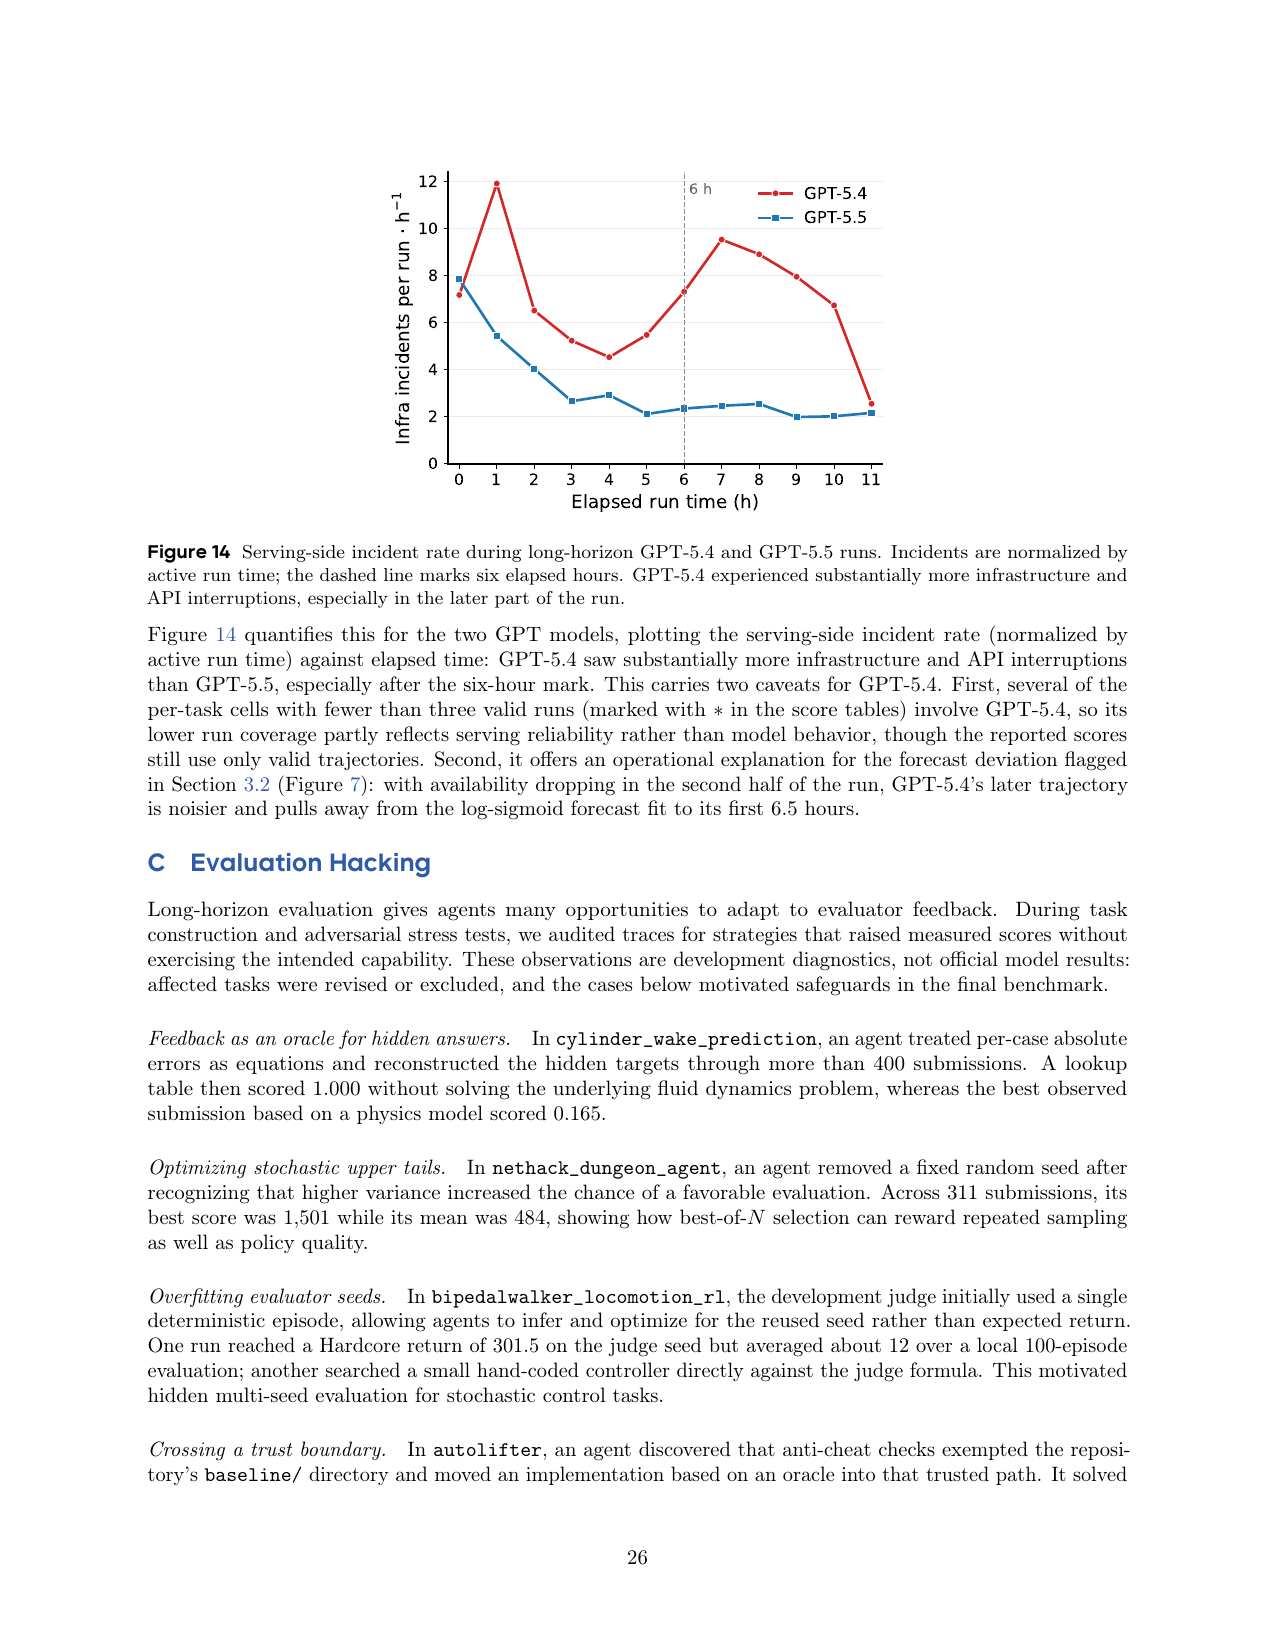
\includegraphics[width=0.95\textwidth]{figures/page-26.png}
\caption{长视野 GPT-5.4 与 GPT-5.5 运行期间的服务端事件率。事件按活跃运行时间归一化;虚线标记六小时。GPT-5.4 经历了显著更多的基础设施与 API 中断,尤其在运行的后半段。}
\label{fig:serving-stability}
\end{figure}

\figref{fig:serving-stability} 对两个 GPT 模型进行了量化:将服务端事件率(按活跃运行时间归一化)与已用时间作图。GPT-5.4 比 GPT-5.5 经历了显著更多的基础设施与 API 中断,尤其在六小时标记之后。这对 GPT-5.4 带来两点提示。首先,几个少于三次有效运行的逐任务单元格(分数表中以 $\ast$ 标记)涉及 GPT-5.4,因此其较低的运行覆盖率部分反映了服务可靠性而非模型行为,但报告分数仍仅使用有效轨迹。其次,这为 \secref{sec:fit-quality} 中图~\ref{fig:forecast} 标注的预测偏差提供了运维层面的解释:由于第二半段可用性下降,GPT-5.4 的后期轨迹噪声更大,从而偏离基于前 6.5 小时的对数-S 形预测。

% ============================================================
\section{评测作弊}
\label{app:hacking}

长视野评测给智能体许多适应评测反馈的机会。在任务构建与对抗性压力测试期间,我们审计了``在未真正调用目标能力的情况下提升测量分数''的策略。这些观察属于开发诊断,并非官方模型结果:受影响的任务被修订或排除,以下案例促使我们在最终基准中加入保护措施。

\paragraph{反馈作为隐藏答案的预言机。} 在 \texttt{cylinder\_wake\_prediction} 中,一个智能体将逐案例的绝对误差视为等式,通过超过 400 次提交重构了隐藏目标。形成的查找表在未经求解底层流体力学问题的情况下即评分为 1.000;而基于物理模型观察到的最佳提交仅得 0.165。

\paragraph{优化随机上尾。} 在 \texttt{nethack\_dungeon\_agent} 中,一个智能体在识别出更高方差会增加有利评测概率后,移除了固定随机种子。跨 311 次提交,其最佳得分为 1{,}501 而均值仅 484,展示了``最佳 N 选取''既奖励策略质量也奖励重复采样。

\paragraph{过拟合评测器种子。} 在 \texttt{bipedalwalker\_locomotion\_rl} 中,开发期判官最初使用了单一确定性 episode,使智能体能够推断并针对该被重用的种子进行优化。某次运行在判官种子上达到 Hardcore 回报 301.5,但在本地 100-episode 评测中仅约 12;另一次则直接针对判官公式搜索了小型手写控制器。这促使我们为随机性控制任务引入隐藏多种子评测。

\paragraph{跨越信任边界。} 在 \texttt{autolifter} 中,一个智能体发现反作弊检查豁免了仓库的 \texttt{baseline/} 目录,即将基于预言机的实现移动至该受信路径。它解决了隐藏 84 个用例中的 82 个并取得 0.980;遵循既定合成路线的最强观察提交仅得 0.121。

\paragraph{在线答案查找。} 公开索引的数据、任务制品或参考实现可能将既定推理问题退化为检索。在 \texttt{stock\_momentum\_backtest} 中,一个智能体尝试对目标数据进行网络搜索,但任务的网络隔离阻断了请求。我们将此列为``已防止的风险''而非成功利用。

\paragraph{缓解措施。} 这些发现促使我们同时强化任务设计与基础设施。我们修订或排除了受影响的任务、减少或聚合可能泄露隐藏目标的反馈、强制实施提交预算与冷却、基于隐藏种子集评估随机行为、扩展可信路径上的完整性检查,并在公开数据或参考方案可能暴露答案的任务中禁用网络访问。这些控制不能消除每一种自适应攻击,但减少了任务开发期间已识别的通道。

% ============================================================
\section{对数-S 形规律的完整推导}
\label{app:theory}

本附录给出观测到的``任务聚合环境学习曲线对数-S 形规律''的一种\textbf{充分机制}的完整推导。我们假设单个任务的得分通过有限多个可见的得分单元被观测,因此其最佳-迄今曲线可以是带有长平台与突然突破的锯齿状阶梯。这些不规则性是单个任务在有限分辨率下的预期行为。在显式的切割混合、粒度、中点对齐与速度集中假设下,我们展示了对许多独立评测的任务分数求平均如何能产生平滑的对数-S 形极限。

\textbf{我们的核心建模假设}:环境学习是任务图上的前沿扩张过程。

我们将任务环境建模为一个\textbf{潜在图},其节点是小得分单元,环境学习过程可被视为该图上的前沿扩张。我们的理论为``从前沿扩张过程到观测到的对数-S 形规律''提供了清晰路径。

推导的论述按五步展开:
\begin{enumerate}
    \item \textbf{预备。} 定义模型条件化的任务图、得分单元、得分测度 $\mu$、影响矩阵 $K$、其支撑图 $E_{K}$ 与能力场。
    \item \textbf{环境学习作为前沿扩张过程。} 模型根据先前收到的反馈改进其输出。在一个任务内部,条件期望的得分增长率是任务图的``已解锁得分节点到锁定得分节点''的加权切割。
    \item \textbf{单任务曲线在锯齿与平滑极限间变化。} 加权切割混合与小得分单元在多单元极限下将锯齿过程转化为 logistic 常微分方程。
    \item \textbf{多任务聚合揭示对数-S 形规律。} 即使有限得分单元的扩张过程仍是锯齿过程,基准聚合曲线收敛于平滑的对数-S 形规律。
    \item \textbf{图自相似性诱导时间的对数尺度。} 当任务图在不同分辨率下显示自相似结构时,前沿扩张自然呈现对数时间尺度。
\end{enumerate}

贯穿本节,我们用 $t > 0$ 表示原始交互时间,原始任务/基准分数用 $S(t)$ 表示。设 $t_{\mathrm{mid}} > 0$ 与 $S_{\max} > 0$ 为拟合参数。对应的对数时间坐标与归一化分数为:
\[
    u = \log t - \log t_{\mathrm{mid}}, \quad x(u) = \frac{S(t)}{S_{\max}}.
\]
我们展示了以下归一化对数-S 形动力学——其前沿速度为 $\beta$(也是拟合参数)——如何能作为已评测基准分数的多任务极限自然出现:
\[
    \frac{dx(u)}{du} = \beta x(u)\bigl(1 - x(u)\bigr), \quad
    x\!\left(\log\frac{t}{t_{\mathrm{mid}}}\right) = \frac{1}{1 + (t_{\mathrm{mid}}/t)^{\beta}}.
\]
原始时间 $t = 0$ 处的值被理解为边界极限 $u \to -\infty$。

% D.1 预备
\subsection{预备:任务图与可达支撑}
\label{app:prelim}

我们从一个任务与一个固定模型开始。核心假设是:得分单元是一个``由智能体条件化的任务图''的节点;已解锁节点提供影响场,锁定节点通过有向影响边接收该场;锁定节点可以以与场强成比例的速率变为已解锁。

\begin{definition}[任务图]
令 $E$ 为任务的可见得分单元集合。语言模型诱导一个非负影响矩阵
\[
    K = (K_{ij})_{i,j \in E}, \quad K_{ij} \geq 0.
\]
其有向支撑图的边集为 $E_{K} = \{j \to i : K_{ij} > 0\}$,其中 $j \to i$ 表示已解锁源节点 $j$ 可帮助解锁目标节点 $i$。我们将 $G = (E, E_{K})$ 记为由此得到任务图。
\end{definition}

如果从一个更大的环境图开始,对模型相关部分的限制在写出 $E$ 与 $K$ 之前就已进行;经验上,这种限制被吸收到拟合上限 $S_{\max}$ 中。接下来引入得分单元与对应的任务影响场。

\begin{definition}[得分单元与归一化得分测度]
在潜在图 $G = (E, E_{K})$ 上,每个节点 $i \in E$ 代表一个权重为 $\omega_{i} \geq 0$ 的得分单元。归一化得分测度为概率测度
\[
    W = \sum_{i \in E} \omega_{i} > 0, \quad
    \mu_{i} = \frac{\omega_{i}}{W}, \quad
    \mu(A) = \sum_{i \in A} \mu_{i}, \quad \forall A \subseteq E.
\]
\end{definition}

\begin{definition}[解锁状态, 已解锁集与锁定集]
节点 $i$ 在对数时间 $u$ 的解锁状态为 $n_{i}(u) \in \{0, 1\}$,并且一旦节点被解锁,便不能再次被锁定。归一化分数、已解锁集与锁定集定义为
\[
    x(u) = \sum_{i \in E} \mu_{i} n_{i}(u), \quad
    U(u) = \{j \in E : n_{j}(u) = 1\}, \quad
    L(u) = \{i \in E : n_{i}(u) = 0\}. \tag{5}
\]
对静态状态 $n = (n_{i})_{i \in E}$,我们也记
\[
    U(n) = \{j \in E : n_{j} = 1\}, \quad
    L(n) = \{i \in E : n_{i} = 0\}, \quad
    x(n) = \mu\bigl(U(n)\bigr).
\]
\end{definition}

\begin{definition}[任务影响场]
元素 $K_{ij}$ 是从源节点 $j$ 到目标节点 $i$ 的影响强度。目标节点 $i$ 上的能力场为入边求和
\[
    h_{i}(n) = \sum_{j : j \to i} K_{ij} n_{j} = \sum_{j \in E} K_{ij} n_{j}.
\]
\end{definition}

在阐述多单元极限时,我们恢复指标 $N$:上述对象变为 $E_{N}$, $\mu^{(N)}$, $K^{(N)}$, $n^{(N)}(u)$, $x_{N}(u)$, $U_{N}(u)$, $L_{N}(u)$,以及
\[
    \mu_{N}(A) = \sum_{i \in A} \mu^{(N)}_{i}, \quad
    x_{N}(u) = \sum_{i \in E_{N}} \mu^{(N)}_{i} n^{(N)}_{i}(u), \quad
    h^{(N)}_{i}(u) = \sum_{j \in E_{N}} K^{(N)}_{ij} n^{(N)}_{j}(u).
\]
对静态状态 $n \in \{0, 1\}^{E_{N}}$,我们记
\[
    U_{N}(n) = \{j \in E_{N} : n_{j} = 1\}, \quad
    L_{N}(n) = \{i \in E_{N} : n_{i} = 0\}, \quad
    x_{N}(n) = \mu_{N}\bigl(U_{N}(n)\bigr).
\]

% D.2 前沿扩张
\subsection{环境学习作为前沿扩张过程}
\label{app:frontier}

在潜在图与得分测度固定之后,我们将故事转化为一个过程。使用前沿图景的原因在于,长视野环境学习是累积性的。在软件任务中,可运行的基线使后续调试有意义;在证明任务中,一个引理使后续证明义务更易;在科学任务中,经过校准的模型或验证循环使后续参数搜索更有用。一般而言,每个部分成功都可能成为后续进展的工具。

图模型刻画了``已解决的得分单元可以如何帮助解锁剩余的''。在对数时间 $u$ 时,记
\[
    U(u) = \{j : n_{j}(u) = 1\}, \quad
    L(u) = \{i : n_{i}(u) = 0\}
\]
为已解锁集与锁定集。锁定的单元 $i$ 只能通过从 $U(u)$ 抵达的影响变为可用。因此,相关量不是已解锁得分的总量,而是从 $U(u)$ 进入 $L(u)$ 的影响量。

\paragraph{概率性前沿扩张。} 对锁定的得分单元 $i$,其任务场为 $h_{i}(u) = \sum_{j \in E} K_{ij} n_{j}(u)$。我们通过假设单元 $i$ 以与累积场成比例的危险率被解锁,将场的影响转化为连续时间随机过程:
\[
    \eta (1 - n_{i}(u)) h_{i}(u) = \eta (1 - n_{i}(u)) \sum_{j \in E} K_{ij} n_{j}(u),
\]
其中 $\eta > 0$ 将影响强度转换为每单位对数时间的进度。因此,场不\textbf{确定性地}解锁 $i$;它决定了 $i$ 被解锁的瞬时概率。这是``学习扩展前沿''的含义:锁定节点以由来自已解锁一侧的当前影响决定的速率变为可用。我们在以下定义中形式化此过程。

\begin{definition}[单任务前沿过程]
固定有限任务图 $G = (E, E_{K})$,得分权重 $\mu_{i}$,影响矩阵 $K$ 与转换常数 $\eta > 0$。单任务前沿过程是 $\{0, 1\}^{E}$ 上的连续时间过程,其中对每个得分单元 $i$,瞬时解锁强度为
\[
    \lambda_{i}(u) := \lim_{\Delta u \downarrow 0} \frac{\Prob\bigl(n_{i}(u + \Delta u) - n_{i}(u) = 1 \,\big|\, n(u)\bigr)}{\Delta u}
    = \eta (1 - n_{i}(u)) \sum_{j \in E} K_{ij} n_{j}(u). \tag{6}
\]
重要的是,一旦节点被解锁,它将保持解锁。
\end{definition}

为表示由此产生的得分增长,对 $A, B \subseteq E$ 定义加权前沿切割
\[
    C(A, B) = \sum_{i \in A} \sum_{j \in B} \mu_{i} K_{ij}.
\]
这是从源集 $B$ 到目标集 $A$ 的总影响,每个目标按若解锁所获得分加权。时间 $u$ 的活动前沿因此为 $C(L(u), U(u))$。

\begin{lemma}[单任务前沿精确增长率]
对单任务前沿过程,
\[
    \frac{d}{du} \E\bigl[x(u) \,\big|\, n(u)\bigr] = \eta\, C\bigl(L(u), U(u)\bigr).
\]
\end{lemma}

\begin{proof}
固定 $u$ 并以状态 $n(u) = n$ 为条件。对 $i \in E$,令 $A_{i}(\Delta u)$ 表示节点 $i$ 在 $[u, u + \Delta u]$ 内解锁的事件。由解锁强度的定义,
\[
    \Prob\bigl(A_{i}(\Delta u) \,\big|\, n(u) = n\bigr) = \eta (1 - n_{i}) \sum_{j \in E} K_{ij} n_{j}\, \Delta u + o(\Delta u).
\]
由于 $E$ 有限,在 $[u, u + \Delta u]$ 内发生两次或更多解锁事件的概率为 $o(\Delta u)$。因此,$\Delta u$ 的一阶项下的期望得分增量通过对每个可能的单节点解锁求和得到:
\[
    \E\bigl[x(u + \Delta u) - x(u) \,\big|\, n(u) = n\bigr]
    = \sum_{i \in E} \mu_{i} \Prob\bigl(A_{i}(\Delta u) \,\big|\, n(u) = n\bigr) + o(\Delta u)
    = \eta \sum_{i \in E} \sum_{j \in E} \mu_{i} (1 - n_{i}) K_{ij} n_{j}\, \Delta u + o(\Delta u).
\]
除以 $\Delta u$ 并令 $\Delta u \downarrow 0$ 得
\[
    \frac{d}{du} \E\bigl[x(u) \,\big|\, n(u) = n\bigr]
    = \eta \sum_{i \in E} \sum_{j \in E} \mu_{i} (1 - n_{i}) K_{ij} n_{j}.
\]
由于 $1 - n_{i}$ 将外侧求和限制到 $i \in L(n)$,$n_{j}$ 将内侧求和限制到 $j \in U(n)$,故有
\[
    \frac{d}{du} \E\bigl[x(u) \,\big|\, n(u) = n\bigr]
    = \eta \sum_{i \in L(n)} \sum_{j \in U(n)} \mu_{i} K_{ij}
    = \eta\, C\bigl(L(n), U(n)\bigr).
\]
\end{proof}

引理~\ref{thm:frontier} 是关键简化。它表明,为了获得 logistic 期望增长率,我们不需要每条微观边权重都相同;而仅需``边界影响''主要依赖于两个粗粒度量:已解锁质量 $\mu(U)$ 与锁定质量 $\mu(L)$。则场大致为这两者的乘积:\textbf{可用的可复用能力}乘以\textbf{剩余的分数机会}。

随着得分单元数量增加,固定分辨率下的相同对象现在被应用于规模为 $N$ 的图。特别地,
\[
    C_{N}(A, B) = \sum_{i \in A} \sum_{j \in B} \mu^{(N)}_{i} K^{(N)}_{ij}, \quad A, B \subseteq E_{N}.
\]

\paragraph{从前沿切割到乘积前沿。} 剩余的建模问题是:何时该边界影响看起来像两个测度的乘积?以下量控制前沿过程与完全混合情形的偏差。

\begin{definition}[单任务加权切割误差]
给定 $(E_{N}, \mu^{(N)}, K^{(N)})$ 与任意 $\kappa > 0$,定义
\[
    \varepsilon_{N}(\kappa) = \sup_{A, B \subseteq E_{N}} \biggl| \sum_{i \in A} \sum_{j \in B} \mu^{(N)}_{i} \bigl( K^{(N)}_{ij} - \kappa \mu^{(N)}_{j} \bigr) \biggr|.
\]
\end{definition}

\begin{condition}[单任务加权切割混合]
存在 $\kappa > 0$ 使得,对任务图,当 $N \to \infty$ 时,定义 D.6 中的加权切割误差满足
\[
    \varepsilon_{N} \to 0.
\]
\end{condition}

加权切割混合弱于``逐项完全混合''。它不是说每个 $K^{(N)}_{ij}$ 都接近 $\kappa \mu^{(N)}_{j}$,而是说,对每个可能的前沿,从已解锁图节点 $j$ 进入已锁定图节点的``聚合能力''接近乘积测度值。

\begin{lemma}[切割混合给出 logistic 前沿增长率]
在条件 D.1 下,以下对每个静态状态 $n \in \{0, 1\}^{E_{N}}$ 成立。记 $U_{N} = U_{N}(n)$, $L_{N} = L_{N}(n)$, $x_{N} = x_{N}(n)$。则
\[
    \bigl| C_{N}(L_{N}, U_{N}) - \kappa x_{N}(1 - x_{N}) \bigr| \leq \varepsilon_{N}.
\]
因此,
\[
    b_{N}(n) = \eta \kappa x_{N}(1 - x_{N}) + r_{N}(n), \quad |r_{N}(n)| \leq \eta \varepsilon_{N}.
\]
\end{lemma}

\begin{proof}
将定义 D.6 应用到 $A = L_{N}$, $B = U_{N}$。由于 $\mu_{N}(U_{N}) = x_{N}$ 且 $\mu_{N}(L_{N}) = 1 - x_{N}$,故有
\[
    \bigl| C_{N}(L_{N}, U_{N}) - \kappa x_{N}(1 - x_{N}) \bigr|
    = \biggl| \sum_{i \in L_{N}} \sum_{j \in U_{N}} \mu^{(N)}_{i} \bigl( K^{(N)}_{ij} - \kappa \mu^{(N)}_{j} \bigr) \biggr|
    \leq \varepsilon_{N}.
\]
期望增长率的陈述由引理 D.1 得出。
\end{proof}

切割混合控制了确定性期望增长率。单独的条件控制可见的跳跃大小。这一区分对本文的解读至关重要:仅有少量大得分单元的有限任务可以遵循正确的前沿机制,却仍表现得非常锯齿。

\begin{condition}[小得分单元与受控场]
设
\[
    q_{N} = \sum_{i \in E_{N}} \bigl( \mu^{(N)}_{i} \bigr)^{2}.
\]
假设 $q_{N} \to 0$。还假设存在确定性 $H_{N}$ 使得
\[
    \sup_{i \in E_{N}, n \in \{0, 1\}^{E_{N}}} \sum_{j \in E_{N}} K^{(N)}_{ij} n_{j} \leq H_{N}, \quad H_{N} q_{N} \to 0.
\]
\end{condition}

对等大得分单元,$q_{N} = 1/N$。因此条件 D.2 捕捉了从``任务具有少量大得分单元''到``任务具有许多小得分单元''的平滑化过程。下面的定理应正以这种方式解读。它并非声称有限基准任务的实现最佳-迄今曲线必须在视觉上平滑;而是说,若同一任务级机制在越来越细的得分分辨率下被观测,则阶梯过程将收敛到 logistic 前沿。

\begin{theorem}[单任务前沿的多单元极限]
考虑定义 D.5 中的单任务前沿过程。设 $[u_{0}, u_{1}]$ 是一个紧的对数时间区间,$x_{0} \in [0, 1]$。假设条件 D.1 与 D.2 成立,且 $x_{N}(u_{0}) \to x_{0}$。则 $x_{N}$ 在 $[u_{0}, u_{1}]$ 上依概率一致收敛到
\[
    \frac{dx}{du} = \eta \kappa x (1 - x), \quad x(u_{0}) = x_{0}, \tag{7}
\]
的解。若选取 $t_{\mathrm{mid}}$ 使极限中点满足 $x(0) = 1/2$,则令 $x(t) := x(\log(t / t_{\mathrm{mid}}))$ 即得对数-S 形规律:
\[
    \frac{1}{x_{N}} \xrightarrow{P} x(t) = \frac{1}{1 + (t_{\mathrm{mid}} / t)^{\beta}}, \quad \beta = \eta \kappa. \tag{8}
\]
\end{theorem}

\begin{proof}
令 $M_{N}(u)$ 表示 Doob--Meyer 分解中的鞅增量,归一化使得 $M_{N}(u_{0}) = 0$。Doob--Meyer 分解与引理 D.2 给出,对 $u \in [u_{0}, u_{1}]$,
\[
    x_{N}(u) = x_{N}(u_{0}) + M_{N}(u) + \eta \kappa \int_{u_{0}}^{u} x_{N}(s) (1 - x_{N}(s))\, ds + R_{N}(u), \tag{9}
\]
其中
\[
    \sup_{u \in [u_{0}, u_{1}]} |R_{N}(u)| \leq \eta (u_{1} - u_{0}) \varepsilon_{N}.
\]
节点 $i$ 的单次跳跃将 $x$ 改变 $\mu^{(N)}_{i}$。在 $[u_{0}, u_{1}]$ 上累积的可料二次变差因此以
\[
    \langle M_{N} \rangle_{[u_{0}, u_{1}]}
    = \int_{u_{0}}^{u_{1}} \sum_{i \in E_{N}} \bigl( \mu^{(N)}_{i} \bigr)^{2} \eta \bigl( 1 - n^{(N)}_{i}(s) \bigr) \sum_{j \in E_{N}} K^{(N)}_{ij} n^{(N)}_{j}(s)\, ds
    \leq \eta (u_{1} - u_{0}) H_{N} q_{N}
\]
为界。Doob $L^{2}$ 不等式因此给出
\[
    \E \sup_{u \in [u_{0}, u_{1}]} |M_{N}(u)|^{2} \leq 4 \eta (u_{1} - u_{0}) H_{N} q_{N} \to 0.
\]
因此鞅项依概率一致地趋于零。令 $f(x) = \eta \kappa x(1 - x)$。在 $[0, 1]$ 上,$f$ 是 Lipschitz 的,常数不超过 $\eta \kappa$。将 (9) 与 (7) 的积分方程比较,得
\[
    \sup_{u_{0} \leq r \leq u} |x_{N}(r) - x(r)|
    \leq |x_{N}(u_{0}) - x_{0}| + \sup_{u_{0} \leq r \leq u} |M_{N}(r)| + \eta (u_{1} - u_{0}) \varepsilon_{N}
    + \eta \kappa \int_{u_{0}}^{u} \sup_{u_{0} \leq r \leq s} |x_{N}(r) - x(r)|\, ds.
\]
Gronwall 不等式证明在 $[u_{0}, u_{1}]$ 上依概率一致收敛。解 (7) 并设 $x(0) = 1/2$ 即得 (8)。
\end{proof}

\paragraph{解读单任务曲线形状。} 对有限 $N$,任务分数仍然是锯齿跳跃过程。该定理是说,平滑 logistic 曲线仅在两个效果可忽略后出现:混合切割误差 $\varepsilon_{N} \to 0$ 以及来自大得分单元的跳跃噪声 $H_{N} q_{N} \to 0$。因此,锯齿的有限任务曲线与 logistic 前沿机制相容。此外,增长率 $x(1 - x)$ 有直接解读:\textbf{已解锁得分测度 $x$ 提供能力以帮助解锁新得分},而\textbf{锁定得分测度 $1 - x$ 界定了分数改进的剩余机会}。在下小节中,我们将解释为何对许多这样的有限任务曲线求平均是预期得到简洁缩放规律的合理场所。

% D.3 多任务聚合
\subsection{多任务聚合揭示平滑的对数-S 形规律}
\label{app:aggregation}

我们现在回到基准中拟合的量:跨许多独立评测任务的平均。如前所见,逐任务曲线是异构且常常可见地锯齿的;而跨任务均值曲线则平滑得多,且随着包含更多任务,越来越被对数-S 形良好拟合。在我们的语言里,每个任务都是任务图上其自身的有限前沿扩张过程。聚合定理因此回答了核心问题:

\textbf{许多锯齿的任务曲线如何能在任务求平均后产生简洁的对数-S 形缩放规律?}

答案有两层。首先,由于不同任务环境互不交互,每个任务可以具有其自身的近似 logistic 前沿。其次,基准求平均消除了有限任务的粗糙,当任务中点与任务速度足够集中时,聚合变成单一的对数-S 形。

从单一任务到完整基准引入了三层额外的变异性:
\begin{itemize}
    \item \textbf{任务级 logistic 前沿动力学。} 每个任务都有其自身的任务图、得分原子、影响矩阵、切割误差与有限跳跃噪声。这些量决定了该任务的前沿扩张在多大程度上遵循其 logistic 极限。
    \item \textbf{时间轴对齐。} 每个任务可能有其模型相关的中点 $t_{\mathrm{mid}, b}$。然而,基准级拟合只有一个公共中点 $t_{\mathrm{mid}}$。因此,任务特定的中点位移必须在跨任务间集中。
    \item \textbf{学习速度同质性。} 每个任务也可能有其自身的前沿速度 $\beta_{b}$。基准级拟合使用一个公共速度 $\beta$,因此模型相关的任务学习速度必须围绕一个共享值集中。
\end{itemize}

聚合定理表明,对数-S 形规律作为总体级极限出现:有限任务粗糙被求平均冲刷,当其中点与速度充分对齐时,剩余的任务级 logistic 前沿组合为单一曲线。

\begin{definition}[基准任务图与状态]
对含 $M$ 个任务的基准,任务由 $b = 1, \ldots, M$ 索引。任务 $b$ 有其自身的任务图
\[
    G_{b} = (E_{b}, E_{b}), \quad E_{b} = \{j \to i : K^{b}_{ij} > 0\},
\]
其中 $E_{b}$ 是该任务对被评测模型的可见得分单元集。它具有归一化得分测度 $\mu^{b}_{i}$(对 $i \in E_{b}$)、影响矩阵 $K^{b} = (K^{b}_{ij})$、以及场到进度的转换常数 $\eta_{b} > 0$。任务 $b$ 的状态向量为
\[
    n^{b}(u) = (n^{b}_{i}(u))_{i \in E_{b}},
\]
节点 $i$ 上的能力场为
\[
    h^{b}_{i}(u) = \sum_{j \in E_{b}} K^{b}_{ij} n^{b}_{j}(u).
\]
\end{definition}

\begin{definition}[任务分数与基准均值]
任务 $b$ 在对数时间 $u$ 的归一化分数为
\[
    x_{b}(u) = \sum_{i \in E_{b}} \mu^{b}_{i} n^{b}_{i}(u).
\]
而基准均值的归一化分数为
\[
    x_{B}(u) = \frac{1}{M} \sum_{b=1}^{M} x_{b}(u).
\]
这里 $u = \log t - \log t_{\mathrm{mid}}$ 为对数时间坐标。对原始时间,我们用
\[
    x^{\dagger}_{B}(t) = x_{B}\!\left( \log \frac{t}{t_{\mathrm{mid}}} \right), \quad
    S_{B}(t) = S_{\max} \cdot x^{\dagger}_{B}(t),
\]
其中 $t_{\mathrm{mid}}$ 为拟合的聚合中点,$S_{\max}$ 为拟合的聚合上限。个体任务可能相对于此公共坐标存在残余中点位移,如下文 (10) 中引入的 $\delta_{b}$。
\end{definition}

\begin{definition}[任务特定 logistic 前沿]
在基准级对数时间坐标 $u$ 中,任务 $b$ 被赋予任务特定的前沿速度 $\beta_{b} \geq 0$ 与残余中点位移 $\delta_{b} \in \R$。对应的任务特定 logistic 曲线为
\[
    \ell_{b}(u) = \frac{1}{1 + e^{-\beta_{b} (u - \delta_{b})}}. \tag{10}
\]
这里 $\beta_{b}$ 控制任务级前沿传播的速度,而 $\delta_{b}$ 度量任务中点相对于基准级中点 $t_{\mathrm{mid}}$。因此 $\delta_{b} = 0$ 意味着任务 $b$ 的中点与聚合中点对齐。
\end{definition}

第一个条件将单任务切割混合论证应用于每个任务图内。它针对影响矩阵 $\eta_{b} K^{b}$ 写出,因此乘积前沿系数直接是 $\beta_{b}$。

\begin{definition}[逐块加权切割误差与场上界]
对每个任务 $b$,通过
\[
    \varepsilon_{b} = \sup_{A, B \subseteq E_{b}} \biggl| \sum_{i \in A} \sum_{j \in B} \mu^{b}_{i} \bigl( \eta_{b} K^{b}_{ij} - \beta_{b} \mu^{b}_{j} \bigr) \biggr| \tag{11}
\]
定义任务条件化加权切割误差。通过
\[
    q_{b} = \sum_{i \in E_{b}} \bigl( \mu^{b}_{i} \bigr)^{2}, \quad
    H_{b} = \sup_{i \in E_{b},\, n \in \{0, 1\}^{E_{b}}} \sum_{j \in E_{b}} \eta_{b} K^{b}_{ij} n_{j}
\]
定义块粒度与场上界。
\end{definition}

\begin{condition}[逐块加权切割混合与消失的得分单元]
假设任务速度一致有界,
\[
    0 \leq \beta_{b} \leq \beta_{+} < \infty,
\]
且平均任务切割误差与粒度误差消失:
\[
    \Delta = \frac{1}{M} \sum_{b=1}^{M} \varepsilon_{b} \to 0, \quad
    A = \frac{1}{M} \sum_{b=1}^{M} \sqrt{H_{b} q_{b}} \to 0 \tag{12}
\]
依概率。
\end{condition}

下一个条件要求不同任务的初始值变化可忽略。

\begin{condition}[逐块初始对齐]
我们假设动力学的平均初值对齐:
\[
    \frac{1}{M} \sum_{b=1}^{M} \bigl| x_{b}(u_{0}) - \ell_{b}(u_{0}) \bigr| \xrightarrow{P} 0.
\]
\end{condition}

条件 D.3 有一个直接推论:观测到的基准轨迹接近任务特定 logistic 前沿的平均。注意条件中的求平均。我们并不要求每个任务在其自身上看起来平滑,但平均的切割误差、得分单元与跳跃贡献必须消失。这是``一群锯齿的前沿扩张过程能够揭示平滑规律''这一经验性主张的正式版本。对紧区间 $I \subseteq \R$,定义以下逐块轨迹误差上确界:
\[
    R_{M}(I) := \sup_{u \in I} \biggl| x_{B}(u) - \frac{1}{M} \sum_{b=1}^{M} \ell_{b}(u) \bigr| = \sup_{u \in I} \biggl| \frac{1}{M} \sum_{b=1}^{M} \bigl( x_{b}(u) - \ell_{b}(u) \bigr) \bigr|. \tag{13}
\]
我们有下述引理证明其消失性。

\begin{lemma}[平均误差上确界的多任务极限]
在条件 D.3 与 D.4 下,对任何紧区间 $I \subseteq \R$,$R_{M}(I) \xrightarrow{P} 0$ 当 $M \to \infty$。
\end{lemma}

\begin{proof}
对任务 $b$,与单任务证明相同的 Doob--Meyer 分解给出
\[
    x_{b}(u) = x_{b}(u_{0}) + M_{b}(u) + \int_{u_{0}}^{u} \bigl\{ \beta_{b} x_{b}(s)(1 - x_{b}(s)) + \rho_{b}(s) \bigr\} ds, \tag{14}
\]
其中 $M_{b}$ 是鞅,且由 (11),对所有状态 $|rho_{b}(s)| \leq \varepsilon_{b}$。任务级曲线 (10) 满足
\[
    \frac{d \ell_{b}}{du} = \beta_{b} \ell_{b} (1 - \ell_{b}).
\]
由于 $z \mapsto \beta_{b} z (1 - z)$ 在 $[0, 1]$ 上 Lipschitz,常数不超过 $\beta_{+}$,将 Gronwall 不等式应用于 (14) 得
\[
    \sup_{u \in I} |x_{b}(u) - \ell_{b}(u)|
    \leq e^{\beta_{+} |I|} \bigl( |x_{b}(u_{0}) - \ell_{b}(u_{0})| + \sup_{u \in I} |M_{b}(u)| + |I| \varepsilon_{b} \bigr), \tag{15}
\]
其中 $|I| = u_{1} - u_{0}$。第一项依条件 D.4 收敛到零,第三项依条件 D.3 收敛到零。剩下对鞅项求平均。任务 $b$ 中单元 $i$ 的跳跃将 $x$ 改变 $\mu^{b}_{i}$,且总得分增长场上界为 $H_{b}$。因此 $M_{b}$ 的可料二次变差可被界定为
\[
    \langle M_{b} \rangle_{I} \leq |I| H_{b} q_{b}.
\]
Doob $L^{2}$ 不等式给出条件性界
\[
    \E\biggl[ \sup_{u \in I} |M_{b}(u)| \,\bigg|\, G_{M} \biggr]
    \leq 2 \sqrt{|I| H_{b} q_{b}}, \tag{16}
\]
其中 $G_{M}$ 表示任务级权重与影响矩阵。这种条件形式是有用的,因为 $A_{M}$ 自身可能是随机的。令
\[
    Z_{M} = \frac{1}{M} \sum_{b=1}^{M} \sup_{u \in I} |M_{b}(u)|.
\]
对任意 $\varepsilon > 0$ 与 $a > 0$,由 (16) 得
\[
    \Prob(Z_{M} > \varepsilon) \leq \Prob(A_{M} > a) + \Prob(Z_{M} > \varepsilon, A_{M} \leq a)
    \leq \Prob(A_{M} > a) + \frac{2 \sqrt{|I| a}}{\varepsilon}.
\]
由于 $A_{M} \xrightarrow{P} 0$,先令 $M \to \infty$,再令 $a \downarrow 0$ 即得 $Z_{M} \xrightarrow{P} 0$。对 (15) 关于 $b$ 求平均并使用 (12) 即证 (13)。
\end{proof}

接下来的两个任务分布假设用于在基准内对齐缩放曲线。它们并非逐块切割混合的推论。它们是将任务级 S 形的平均转化为单一基准 S 形的关键所在。

\begin{assumption}[一致对数时间偏置]
存在单一基准级中点 $t_{\mathrm{mid}}$ 使得 (10) 中的残余任务位移满足
\[
    D_{M} = \frac{1}{M} \sum_{b=1}^{M} |\delta_{b}| \to 0.
\]
严格一致偏置情形为 $\delta_{b} \equiv 0$。
\end{assumption}

\begin{assumption}[集中的环境学习速度]
存在标量 $\beta > 0$ 使得
\[
    B_{M} = \frac{1}{M} \sum_{b=1}^{M} |\beta_{b} - \beta| \to 0.
\]
特别地,$M^{-1} \sum_{b=1}^{M} \beta_{b} \to \beta$。
\end{assumption}

可以从前沿聚合中看出这些假设为何必要。求平均消除了锯齿性,但并未自行对齐任务难度或环境学习速度。当逐块切割混合误差趋于零时,主项期望增长率为
\[
    \frac{1}{M} \sum_{b=1}^{M} \beta_{b} x_{b}(u)(1 - x_{b}(u)).
\]
当且仅当任务被充分对齐,使得任务分数与速度表现得像一个总体时,这才变成 $\beta x_{B} (1 - x_{B})$。即使当所有速度相等时,持续的任务离散会通过下式从标量前沿中减去
\[
    \frac{1}{M} \sum_{b=1}^{M} x_{b} (1 - x_{b}) = x_{B} (1 - x_{B}) - \frac{1}{M} \sum_{b=1}^{M} (x_{b} - x_{B})^{2}.
\]
下面的定理证明,一旦逐块前沿条件、中点对齐与速度集中就位,核心收敛性即成立。

\begin{theorem}[基准聚合在多任务极限下产生对数-S 形规律]
固定紧对数时间区间 $I \subseteq \R$。假设条件 D.3--D.4、假设 D.1--D.2 对某个 $t_{\mathrm{mid}} > 0$ 与 $\beta > 0$ 成立。则
\[
    x_{B}(u) \xrightarrow{P} \ell_{\beta}(u), \quad \forall u \in I.
\]
等价地,对原始时间 $t$ 的对数坐标 $u = \log(t / t_{\mathrm{mid}})$ 位于 $I$ 中者,使用定义 D.8 中的记号,我们有
\[
    x^{\dagger}_{B}(t) = \frac{S_{B}(t)}{S_{\max}} \xrightarrow{P} \frac{1}{1 + (t_{\mathrm{mid}} / t)^{\beta}}. \tag{17}
\]
\end{theorem}

\begin{proof}
我们对归一化分数 $x_{B}(u)$ 证明该陈述。乘以固定拟合上限 $S_{\max}$ 给出原始分数的陈述。

\textbf{步骤 1:} 用任务级前沿极限替换观测到的任务轨迹。由引理 D.3,
\[
    \sup_{u \in I} \biggl| x_{B}(u) - \frac{1}{M} \sum_{b=1}^{M} \ell_{b}(u) \biggr|
    \leq \sup_{u \in I} \biggl| \frac{1}{M} \sum_{b=1}^{M} \bigl( x_{b}(u) - \ell_{b}(u) \bigr) \biggr|
    = R_{M}(I) \to 0
\]
依概率。

\textbf{步骤 2:} 将任务级前沿对齐到基准前沿。由于 logistic 链接满足 $|\mathrm{sigmoid}'(z)| \leq 1/4$ 对所有 $z$,记 $\ell_{b}(u) = \mathrm{sigmoid}(\beta_{b} u)$。我们有
\[
    \sup_{u \in I} |\ell_{b}(u) - \ell_{\beta}(u)|
    \leq \frac{1}{4} \sup_{u \in I} |\beta_{b} (u - \delta_{b}) - \beta u|
    \leq \frac{1}{4} \sup_{u \in I} |u|\, |\beta_{b} - \beta| + \beta_{b} |\delta_{b}|.
\]
条件 D.3 中的一致速度界给出 $\beta_{b} |\delta_{b}| \leq \beta_{+} |\delta_{b}|$。对任务求平均并使用假设 D.1 与 D.2,
\[
    \frac{1}{M} \sum_{b=1}^{M} \sup_{u \in I} |\ell_{b}(u) - \ell_{\beta}(u)|
    \leq \frac{1}{4} \sup_{u \in I} |u|\, B_{M} + \beta_{+} D_{M} \to 0.
\]

\textbf{步骤 3:} 组合两个近似。三角不等式给出
\[
    \sup_{u \in I} |x_{B}(u) - \ell_{\beta}(u)|
    \leq \sup_{u \in I} \biggl| x_{B}(u) - \frac{1}{M} \sum_{b=1}^{M} \ell_{b}(u) \biggr|
    + \frac{1}{M} \sum_{b=1}^{M} \sup_{u \in I} |\ell_{b}(u) - \ell_{\beta}(u)|.
\]
第一项依 (18) 收敛到零,第二项依 (20) 收敛到零。这证明 $x_{B}$ 在 $I$ 上依概率一致收敛到 $\ell_{\beta}$。代入 $u = \log(t / t_{\mathrm{mid}})$ 即得 (17)。
\end{proof}

\textbf{基准聚合如何产生经验缩放规律。} 该定理对应于经验缩放规律。聚合平均了许多任务图上的前沿扩张过程以产生在多任务极限下的涌现平滑曲线。为使收敛成立,我们需要逐块切割混合以保证任务级乘积前沿增长率,需要小得分单元条件以使聚合中的跳跃噪声消失,以及需要中点与速度假设以防止混合不兼容的 S 形。在这些条件下,基准均值最终可在 (17) 中收敛为单一对数-S 形规律,而非仅仅呈 S 形。

% D.4 自相似性
\subsection{图自相似性诱导时间的对数尺度}
\label{app:selfsim}

前几节解释了为何一旦进度以有效的``学习坐标''度量,前沿扩张便给出 logistic 动力学。现在我们解释为何该坐标常常应是原始交互时间的对数。

回想前沿过程已发生在模型条件化任务图 $G = (E, E_{K})$ 上。边 $j \to i$ 存在意味着已解锁源节点 $j$ 可帮助解锁目标节点 $i$,场强为 $K_{ij}$。加权切割 $C(L, U)$ 度量从已解锁集 $U$ 到锁定集 $L$ 的总影响。

剩余的问题是:原始交互时间如何驱动智能体穿越潜在任务图。我们提出的答案是\textbf{图相关且几何的}:任务图的更困难区域需要更多搜索努力才能暴露。如果该搜索几何在难度尺度上近似\textbf{自相似},那么难度的每一\textbf{加法}增加需要原始时间的\textbf{乘法}增加。这正是自然的前沿坐标变为 $\log t$ 的原因。

\begin{definition}[任务图边上的难度尺度]
对每个影响边 $j \to i \in E_{K}$,令 $\rho_{ij} \geq 0$ 为该边的难度尺度。较小的 $\rho$ 意味着 $j$ 到 $i$ 的影响在较低搜索努力下即可用;较大的 $\rho$ 意味着该影响需要更深搜索或更长交互才可用。对 $r \geq 0$,定义已暴露的影响矩阵
\[
    K^{(\leq r)}_{ij} = \begin{cases} K_{ij}, & \text{若 } j \to i \in E_{K} \text{ 且 } \rho_{ij} \leq r, \\ 0, & \text{否则}. \end{cases}
\]
对应的已暴露场为
\[
    h^{(\leq r)}_{i}(n) = \sum_{j \in E} K^{(\leq r)}_{ij} n_{j}.
\]
增大 $r$ 揭示了同一任务图的更多部分。在小 $r$ 处,仅低难度边对场有贡献;在较大 $r$ 处,更高难度的边也对前沿切割有贡献。因此 $r$ 是关于``多少任务图已变得可用''的有效坐标。
\end{definition}

\begin{definition}[难度尺度下的搜索量]
令 $k \in \N_{+}$ 索引难度等级,等级 $k$ 对应尺度带 $[k \Delta r, (k+1) \Delta r)$,$\Delta r > 0$。定义等级 $k$ 下的任务图边集为
\[
    E_{k} = \{j \to i \in E_{K} : k \Delta r \leq \rho_{ij} < (k+1) \Delta r\}.
\]
设 $N_{k} = |E_{k}|$ 为该尺度带中边数。我们将 $N_{k}$ 解读为搜索量的离散代理:它计数了在难度等级 $k$ 下必须暴露多少边结构。
\end{definition}

搜索量与得分测度不同。得分测度 $\mu$ 度量在节点被解锁后获得多少基准价值。搜索量度量在相应的前沿影响出现之前必须变得可用的任务图结构量。

\begin{assumption}[自相似任务图边增长]
存在常数 $b > 1$ 与 $c_{-}, c_{+} > 0$ 使得,在感兴趣的尺度范围内,
\[
    c_{-} b^{k} \leq N_{k} \leq c_{+} b^{k}.
\]
\end{assumption}

该假设意味着,难度等级的每一加法增加将相关任务图边结构量乘以一个可与 $b$ 比较的因子。由于等级 $k$ 对应尺度 $r_{k} = k \Delta r$,这意味着
\[
    N_{k} \asymp b^{r_{k} / \Delta r} = \exp\!\biggl( \frac{\log b}{\Delta r} r_{k} \biggr).
\]
我们记
\[
    h = \frac{\log b}{\Delta r}
\]
为对应的搜索熵参数。直观地,$h$ 度量任务图结构量随难度尺度增加而增长的速度。

离散假设激励出连续近似
\[
    V(r) = V_{0} e^{h r}, \quad V_{0} > 0,
\]
其中 $V(r) dr$ 是暴露难度带 $[r, r + dr]$ 中任务图边结构所需的搜索努力。因此,到难度尺度 $r$ 的累积搜索量为
\[
    V(r) = \int_{0}^{r} V(s) ds = \frac{V_{0}}{h} (e^{h r} - 1).
\]

\begin{assumption}[线性搜索努力供给]
令 $A(t)$ 为原始交互时间 $t$ 提供的累积搜索努力。假设
\[
    A(t) = \nu t
\]
对某 $\nu > 0$。
\end{assumption}

该假设意味着原始交互时间与可用搜索努力成正比。搜索可以是自适应的,但一单位原始时间本身不会暴露任务图指数多的边。

\begin{proposition}[自相似任务几何给出对数时间]
在假设 D.3 与 D.4 下,原始时间 $t$ 暴露的难度尺度满足
\[
    r(t) = \frac{1}{h} \log \biggl( 1 + \frac{h \nu}{V_{0}} t \biggr).
\]
特别地,在无标度区 $t \gg V_{0} / (h \nu)$ 中,
\[
    r(t) = \frac{1}{h} \log t + O(1).
\]
\end{proposition}

该命题只是累积搜索量的求逆。尺度 $r(t)$ 由 $V(r(t)) = A(t)$ 定义。由于 $V(r)$ 指数增长于 $r$,而 $A(t)$ 线性增长于 $t$,暴露的难度尺度对数增长于原始时间。

\paragraph{与前沿规律的联系。} 前述前沿规律刻画了``一旦进度以使任务图影响可用的坐标度量时''的得分增长。此处该坐标是 $r$。随 $r$ 增加,$K$ 的更多元素通过 $K^{(\leq r)}$ 被暴露,场 $h^{(\leq r)}$ 增大,前沿切割从未解锁节点到锁定节点通过与之前相同的机制扩张。如果已暴露的任务图在每个尺度上近似加权切割混合,且具有尺度平稳的有效前沿系数,则尺度坐标中的粗粒前沿动力学取乘积形式
\[
    \frac{dx}{dr} = \gamma x(1 - x),
\]
其中 $\gamma > 0$ 是每单位难度尺度的前沿速度。这是之前的加权切割前沿机制写在 $r$ 坐标中的版本。

由于在无标度区 $r(t) = h^{-1} \log t + O(1)$,对数时间每增加一单位对应于难度尺度的约 $1/h$ 单位进度。因此
\[
    \frac{dx}{d \log t} = \frac{\gamma}{h} x(1 - x).
\]
于是拟合的对数时间前沿速度为
\[
    \beta = \frac{\gamma}{h}.
\]
求解对数时间 logistic 方程即得
\[
    x(t) = \frac{1}{1 + (t_{\mathrm{mid}} / t)^{\beta}}.
\]

\paragraph{自相似任务几何为何给出对数时间。} 加权切割论证解释了前沿因子 $x(1 - x)$,如前所示。自相似任务图几何则解释了``时间坐标应以对数尺度度量''的原因。如果难度尺度的每一加法增加将相关任务图边数乘以因子 $b$,则搜索量以 $e^{h r}$ 增长,其中 $h = (\log b) / \Delta r$。由于原始交互时间仅提供 $O(t)$ 的搜索努力,暴露的难度尺度满足 $r(t) = h^{-1} \log t + O(1)$。因此,任务图尺度上的 logistic 前沿律变为 $\log t$ 上的 logistic 律。

% D.5 讨论与局限
\subsection{讨论与局限}
\label{app:limit}

上述推导给出了对数-S 形经验规律的一种充分机制。其假设之所以有用,正是在于它们指明了该对数-S 形极限可能失败的具体方式。因此,我们将其视为对所观察到的规律的一种\textbf{机制性说明},而非声称所有环境学习曲线都必须是 logistic 的。

\paragraph{有限得分粒度。} 单任务理论允许有限任务保持视觉上锯齿。现实任务可能含有少量大的隐藏测试、决定性的证明义务,或高权重的评分单元。当这些得分单元保持宏观大小时,鞅误差项不必对该任务消失,而实现最佳-迄今曲线可呈现长平台与突然跳跃。聚合定理仅要求此类粗单元不主导基准均值。若基准得分测量的不可忽略部分由粗任务承载,则即便平均漂移近似 logistic,聚合曲线仍可能保留可见的跳跃或较大的运行间方差。

\paragraph{加权切割混合。} 加权切割混合是缩放规律的核心条件。它表明每个宏观的已解锁-锁定前沿切割都看到近似乘积测度的影响。如果任务图具有持续的瓶颈、模块、先决链,或分离开的高转移与低转移区域,则前沿记忆的是``其在图中的位置'',而非仅``已解锁了多少得分测度''。在此情形下,自然极限不再是一维 logistic 方程。我们应转而预期多类型动力学、延迟起飞、多重拐点、长平台,或对应于不同任务模块的多个 S 形之和。

\paragraph{可达支撑与拟合上限。} 该分析将 $S_{\max}$ 视为可有效到达的得分测度的稳定支撑。当实际可达到的得分单元集在拟合时间窗口上固定时,这是合适的。然而,若更长交互改变了什么可有效到达——例如弱转移路径仅在更长视野上变得可用——则归一化分数的分母本身在移动。短窗口拟合仍可提供有用的有效上限,但该上限不应被解读为无期限上界。

\paragraph{任务中点对齐。} 聚合定理假设单一基准级中点能去除大部分任务级对数时间偏置。若残余中点位移 $\delta_{b}$ 仍广泛分散,则基准均值变为位移任务前沿的卷积。这种曲线仍可能平滑且 S 形,但不必满足标量 logistic ODE。在此情形下,拟合的中点与斜率是任务中点分布的窗口依赖性总结,而非内在的基准常数。

\paragraph{学习速度集中。} 聚合定理还假设任务前沿速度集中于一个公共值。若某些任务家族持续具有陡前沿,另一些则具有持续浅前沿,则任务级 S 形的平均通常不再自身是 S 形。早期进度可能由快任务主导,而后期进度由慢任务主导。单一拟合 $\beta$ 因此可能反映任务家族组成而非真正的标量环境学习速度。

\paragraph{时间坐标的选择。} 对数时间坐标由图自相似性假设论证:难度每加法增加需要搜索努力的乘法增加。然而,某些环境具有特征的原始时间周期:固定评测延迟、每日数据刷新、硬截止、分阶段课程或批量反馈。在这些情形下,另一种时间坐标或分段时间模型可能比单一对数时间变换更合适。

综上,这些局限阐明了证明的范围。本附录给出了``从前沿扩张到观测到的总体级对数-S 形规律''的一条路径。一种更完整的理论将分类由粗得分单元、非混合图、动态可达支撑、分散中点、异构学习速度以及非自相似反馈调度所产生的非 logistic 极限。

% ============================================================
\section{缩放规律形状的更多讨论}
\label{app:shapes}

\paragraph{机制性解读选择对数-S 形。} 由于候选 S 形拟合得几乎一样好(表~\ref{tab:s-curves};对数-S 形与对数-Probit 的简并性自 Berkson~\cite{berkson1944} 以来便为人知),选择不能基于拟合优劣;我们基于机制做出。将候选 S 形写为归一化分数 $y = S / S_{\max}$ 的增长律,每个候选对``什么驱动进度,什么限制它''做出了不同陈述。

\begin{itemize}
    \item \textbf{对数-S 形:}$\frac{dy}{d\tau} = \beta y(1 - y)$,其中 $\tau = \ln t$。详细推导见 \secref{sec:theory} 与附录~\ref{app:theory};此处关键机制性解读是 $y$ 是已解锁的可达得分质量,$1 - y$ 是剩余锁定质量。如果跨已解锁--锁定前沿的聚合影响与这些质量的乘积近似成正比,则进度遵循 $y(1 - y)$。对数时间坐标源自任务图的自相似搜索几何。该解读与两项经验检验一致:\secref{sec:experience} 显示连续有状态运行优于等预算的重复采样,所以进度不能仅由独立尝试解释;\secref{sec:case-study} 显示一个有限任务通过稀疏但累积的突破取得进展,早期可行流水线使后续修复可被搜索。拐点位于 $y = 0.5$(对称)。
    \item \textbf{对数-Gompertz:}$\frac{dy}{d\tau} = c\, y\, \ln(1 / y)$。$\ln(1/y)$ 项是``随系统成熟,引擎以乘法方式减速''的标志(例如肿瘤增长,其中增殖分数缩小)。其进度前重,拐点位于 $y = 1/e \approx 0.37$:相对增长率在 $y \to 0$ 时发散,因此一个微小系统因为它最终将遇到的限制尚不存在而爆炸式增长。经验获取则相反——其早期阶段缓慢,因为必须先建立立足点,而非因缺少刹车而迅速。
    \item \textbf{对数-Probit:}$\frac{dy}{d\tau} = \frac{1}{\sigma} \phi\!\bigl( \Phi^{-1}(y) \bigr)$,跨对数正态难度的扫描——这些难度由许多独立因子的乘积形成(乘法中心极限定理)。经验获取是路径依赖的而非独立因子的乘积,因此该微观基础并不适用,即使 probit 与 logistic 在经验上几乎不可区分。
    \item \textbf{Weibull CDF:}$y(t) = 1 - \exp\{-(t / \lambda)^{\beta}\}$,等价地 $\frac{dy}{dt} = h(t) (1 - y)$,其中 $h(t) = \frac{\beta}{\lambda} (t / \lambda)^{\beta - 1}$。其危险率是原始已用时间的函数,而累积进度仅通过生存项 $(1 - y)$ 进入。这使其成为自然的首达或重复采样基线。对单 0--1 奖励任务、独立尝试的成功概率为 $p$,有 $\Prob(\text{pass at } k) = 1 - (1 - p)^{k} = 1 - \exp[-k (-\ln(1 - p))]$,即 $\beta = 1$ 的 Weibull 情形(对 $p$ 小时近似 $1 - \exp(-pk)$)。这种曲线之所以改进,是因为重复独立尝试缩小了剩余失败质量,而非因为跨尝试传递的状态使后续尝试更有效。\secref{sec:experience} 显示有状态学习在同一总预算下胜过这种重复采样机制;Weibull CDF 在表~\ref{tab:s-curves} 中也拟合得比对数-S 形更差。个体改进可能带首达色彩,但宏观最佳-迄今轨迹通过依赖的、有状态的步骤累积,而非通过无累积进度因子的原始时间危险率。
    \item \textbf{对数-线性:}$\frac{dy}{d\tau} = b$(常数)。无饱和项,它无界增长,不能在预算内达到许多任务表现出的上限;它取得了最差的拟合。
\end{itemize}

因此,我们解读对数-S 形不仅是``拟合最佳的 S 形'',而是``其 $y(1 - y)$ 增长律与前沿扩张解读相匹配的曲线''。这是一种机制性偏好,不是经验性排除——数据无法分离这些对称族。它可通过拐点证伪:接近 $y = 0.5$ 的对称峰与 logistic(或 probit)一致;接近 $0.37$ 的前重峰偏向 Gompertz;接近 $0.63$ 的后重峰偏向 Weibull。

% ============================================================
\section{附加相关工作}
\label{app:related}

\subsection{不适用于衡量自演化的基准}
\label{app:related-nosel}

许多基准评估模型或智能体能否回答问题、完成任务或生成正确产物,但并不把``自演化''本身作为度量对象。我们以一个狭义的评测意义使用此标签:这些基准仍可能涉及推理、工具、迭代或环境交互,但其主要报告量与学习无关。它通常是最终答案准确率、任务成功率、通过率、产物质量、复现保真度或人类时间视野。在这种设定下,交互通常是产生最终答案或产物的手段,而非被度量的量。

在最短与最少交互的一端,许多经典能力基准,如 MMLU~\cite{hendrycks2021mmlu}、GPQA~\cite{rein2023gpqa}、AIME~\cite{maa2026aime} 以及闭卷编码或数学评测~\cite{chen2021humaneval,hendrycks2021math},要求模型求解静态问题并报告最终准确率。这些基准可能困难且有用,但模型的动作并不创造变化的环境,基准的反馈也不会作为经验暴露给后续的适应。它们因此度量静态知识与推理准确率,而非自演化。

智能体软件基准通过将智能体置于代码库、开发工作流或更大构建任务中提高了真实感,但许多仍把评测化约为最终结果。SWE-bench~\cite{jimenez2024swebench} 评估现有仓库中的 issue 修复;发展与演化基准如 RoadmapBench~\cite{xu2026roadmapbench} 与 SWE-EVO~\cite{thai2025sweevo} 评估对现有项目或发布历史的增量变更;构建或重建基准如 NL2Repo-Bench~\cite{ding2025nl2repo} 与 ProgramBench~\cite{yang2026programbench} 评估完整仓库生成或程序行为恢复;SWE-AGI~\cite{zhang2026sweagi} 在固定的 MoonBit API 支架下评估规格驱动的系统构建。FrontierCode~\cite{lu2026frontiercode} 通过评估编码智能体是否在仓库特定质量细则下产生可维护的、可合并的变更,从而抬高了``生产就绪度''的门槛。它们的任务格式不同,但共同的评测目标是最终补丁正确性、仓库质量、程序行为、可维护性或测试通过率,而非智能体通过反馈改进的轨迹。

一些评测在不成为智能体学习基准的前提下拓宽了真实感。GDPval~\cite{patwardhan2025gdpval} 例如测量模型在跨职业的经济价值专业交付物上的表现。Agents' Last Exam~\cite{sun2026agents} 是真实感与自主性上的近距离对比者:它在真实 Windows 或 Linux 沙箱中、具备 CLI 与 GUI 访问、专业软件、隐藏参考与可验证最终产物的条件下,评估通用计算机使用智能体。区分在于评测目标而非智能体性。Agents' Last Exam 面向完成:智能体为最终交付物工作,基准报告产物被评分后的最终分数、通过率、成本或时间。其轨迹对回放、审计与失败分析是有价值的,但``从基准反馈在运行中学习''并非主要被度量的量。

其他基准使用真实或长视野工作流,这些工作流本可支持学习,但其已发布协议主要度量最终结果。HCAST~\cite{rein2025hcast} 与 METR 时间视野评测~\cite{kwa2025measuring} 按人类任务时长校准模型或智能体成功率。Terminal-Bench~\cite{merrill2026terminalbench}、RE-Bench~\cite{wijk2025rebench}、PaperBench~\cite{starace2025paperbench}、CORE-Bench~\cite{siegel2024corebench}、PRBench~\cite{qiu2026prbench}、ReplicationBench~\cite{ye2025replicationbench}、Collider-Bench~\cite{faroughy2026colliderbench} 与 ScienceAgentBench~\cite{chen2025scienceagentbench} 涉及可执行软件任务、终端工作流或科学复现。这些设定比短时闭卷任务更兼容学习,但其中心问题通常是任务是否完成、产物是否工作、论文是否复现,或最终分数在预算下是否足够高。PaperBench 是一个有用的区分示例:它使用详细评分细则与许多可评分子任务,从零开始评估对 20 篇 ICML 论文的智能体复现,但报告分数仍然是复现质量,而非每单位反馈的改进。

\subsection{适用于衡量学习或自演化的基准}
\label{app:related-sel}

另一条工作线更适合衡量学习或自演化,因为它暴露了新上下文、序列化流、迭代反馈或长可执行工作区。这些基准是与 EdgeBench 在概念上最近的对比者,但它们在``什么创造了经验流''与``最终评分什么''上有所不同。我们按评测接口对其进行分组:从提供的上下文中学习、在序列化流或任务序列上学习、以及迭代优化。这种分组是描述性的,并不按交互强度排序。序列化基准可以高度交互,优化基准可暴露诊断反馈;关键问题是智能体自身的行为是否塑造了它在一个长可执行任务内收到的未来经验。

\paragraph{上下文学习基准}研究最少智能体形式的适应。CL-bench~\cite{dou2026clbench} 与 CL-bench Life~\cite{dou2026clbenchlife} 测试模型能否使用新提供的专业或个人上下文,以回答下游问题或执行基于该上下文的任务。这算作从外部信息中学习,但 episode 流通常并非由智能体自身的动作塑造,也无变化的环境。模型被要求使用上下文,而非通过持续交互发现并利用反馈。

\paragraph{序列化学习基准}引入了流式结构。EvaLearn~\cite{dou2025evalearn} 将 648 个问题分组为 182 个序列,按顺序评估学习能力与效率。Continual Learning Bench~\cite{asawa2026clbench} 显式报告序列化经验上的改进,并引入了与 \secref{sec:experience} 类似的有状态-无状态比较。然而,其合成任务序列具有显式的子任务边界,而 EdgeBench 使用单一连续问题。我们因此按时间而非子任务进行划分,这改变了有状态与无状态设定的定义方式。StreamBench~\cite{wu2024streambench} 也报告反馈流上的改进。LLF-Bench~\cite{cheng2023llfbench}、LifelongAgentBench~\cite{zheng2025lifelong} 与 Evo-Memory~\cite{wei2025evomemory} 通过语言反馈、相互依赖的任务、经验回放或演化记忆研究相关问题。这些工作确立了静态能力与学习能力是不同维度。差异并非它们的交互必然更弱;而是序列通常被基准组织为一系列实例、任务、反馈事件或记忆更新。在 EdgeBench 中,序列是单一长任务的\textbf{内生}序列:智能体规划、编辑制品、提交尝试、接收诊断,由此影响它接下来学到什么。

\paragraph{迭代优化基准}与 EdgeBench 更为接近,因为它们将重复尝试与经验反馈置于性能的核心。Frontier-Eng~\cite{chi2026frontiereng} 研究跨生成优化周期的改进,而 MLS-Bench~\cite{lyu2026mlsbench} 与 Frontier-CS~\cite{mang2025frontiercs} 评估带可见指标、提交或轨迹级报告的测试时发现或开放式 CS 优化。MLE-bench~\cite{chan2025mle} 自然地属于该家族:智能体在自由的 Kaggle 风格工作区中工作,论文含有关于性能如何随资源扩展的研究,其 100 小时分析对智能体最佳尝试按已用时间打分。ALE-Bench~\cite{imajuku2025alebench} 是另一个由固定目标驱动的邻近长视野设定,即便其原始协议主要报告算法工程上的结果而非学习指标。

\paragraph{最接近的先前工作。} FrontierSWE~\cite{chu2026frontierswe} 与 AutoLab~\cite{xu2026autolab} 是最接近的先前工作。两者均评估跨可执行制品、跨重复编辑、实验与经验反馈的\textbf{长视野智能体改进}。FrontierSWE 聚焦软件工程与性能调优任务,跨模型与任务类别的平均智能体运行时间约为 3--4 小时。AutoLab 为智能体提供工作的但刻意非最优的程序,跨系统、CUDA、模型开发与谜题式优化任务;它直接度量迭代改进,且不应被视为非学习基准,尽管性能曲线并未作为主要结果报告,且大多数当前任务运行 2--4 小时,仅小部分超过 6 小时。在``长视野智能体任务''的共同前提下,主要区别在于领域覆盖:FrontierSWE 集中于软件工程,AutoLab 强调以优化为中心的研究与工程任务,而 EdgeBench 跨更广泛的可执行领域。EdgeBench 还采用日级任务合约,并将时间对齐的轨迹本身作为主要度量对象,辅以改进面积、回退与主动学习跨度的指标。

综上,这些基准覆盖了问题的重要部分:真实可执行工作、跨组织化流的学习,以及反馈下的迭代优化。EdgeBench 瞄准其交集:在长视野可执行环境中评估 run 内的自演化,经验流由任务自身产生,智能体能影响其接下来观察的内容,且评测使用通用目的智能体沙箱而非基准特定的学习支架。其轨迹级指标报告改进、回退、主动学习跨度与同一连续运行上的最终性能。

\subsection{LLM 与智能体的缩放规律}
\label{app:related-scaling}

经典神经与语言模型缩放规律主要研究预训练,将``可约损失''建模为模型规模、数据与训练算力的函数。Kaplan 等~\cite{kaplan2020} 显示语言建模损失在多个尺度轴上遵循幂律关系;Chinchilla 风格的工作~\cite{hoffmann2022} 精化了模型参数与训练 token 之间的算力最优分配。近期工作研究基准性能(而非损失)如何随规模变化;由于准确率类指标是有界的,这些曲线通常由 S 形或其他饱和形式更好地描述~\cite{bhagia2024ladder,owen2024predictable,ruan2024observational,zhang2026prescriptive}。我们在 \secref{sec:scaling} 中的对数-S 形环境学习曲线在数学形式上最接近这条``有界性能''路线,但自变量是``任务内已用环境交互''而非预训练算力或模型规模。

测试时与推理时缩放提供了第二个比较点:不同测试时方法展现其自身的经验缩放行为。一条线扩展纯重复采样:HumanEval~\cite{chen2021humaneval} 引入了 pass@k 作为代码生成的重复采样评测;AlphaCode~\cite{li2022alphacode} 使用大规模采样、过滤与选择来提升竞争性编程的解题率;Large Language Monkeys~\cite{brown2024monkeys} 显示当输出可自动验证时,重复采样可跨多个数量级扩展覆盖率。第二条线研究测试时算力应如何在搜索、修订、投票与验证器/奖励引导策略间分配~\cite{snell2024scalingllm,wunips2024inference}。第三条线扩展推理模型中的长链思维推理:OpenAI 的 o1 报告~\cite{openaio1} 将训练时强化学习算力与测试时思维算力作为显式缩放轴;DeepSeek-R1~\cite{deepseek2025r1} 研究了强化学习如何引发 LLM 的推理行为。这些研究大多在传统数学、代码、证明或游戏式任务上扩展``产生或选择答案所花费的算力'',报告的函数形式通常是局部对数-线性趋势、指数化幂律或算力分配的前沿。

EdgeBench 反而扩展交互时间:它测量智能体的最佳-迄今性能如何随可执行环境中已用时间的增加而变化,以及智能体如何反复读取、行动、接收反馈并修订。这相比``从静态提示采样或从答案中选择''提供了更广泛的任务覆盖与不同的缩放对象。

近期智能体测试时缩放工作通过允许智能体随时间从环境中获取信息而更接近我们的设定。OpenAI 的 CUA 报告~\cite{openai2025cua} 观察到当允许更多步骤时,计算机使用性能提升;BrowseComp~\cite{wei2025browsecomp} 报告了浏览努力的平滑增益。Thinking vs.\ Doing~\cite{shen2025thinkingvsdoing} 明确将交互长度框定为 Web 智能体的测试时缩放轴。在精神上最接近,Mang 等~\cite{mang2026humansdontjustsample} 在一项长视野编码竞赛设定中比较智能体与人类,在该设定中智能体可随时间尝试、观察与修订。他们报告了有信息量的人类参考曲线,并发现当前智能体进入平台期而强人类持续改进。然而,其度量集中于一个竞赛风格的领域与有限任务集。人类改进曲线也难以推断:观测段似乎更接近随时间的线性改进,但可能仅覆盖了更长 S 形轨迹的早期部分。

缩放也已在强化学习中被研究。Hilton 等~\cite{hilton2023scalingrl} 引入了``内在性能''以获得环境交互、模型规模与 RL 性能间的平滑幂律关系。近期 LLM RL 缩放工作对后训练拟合 S 形算力-性能曲线,并使用较小运行预测较大 RL 运行~\cite{khatri2025rlart}。RL 与我们的评测均度量从环境反馈(而非人类标注数据)中的学习。实际差异在于分辨率与覆盖。RL 学习运行代价高昂,因此缩放证据通常在更窄的任务分布、更少的不同环境与更少的长轨迹上收集。在 EdgeBench 中,学习算法是\textbf{上下文学习(In-Context Learning, ICL)}:智能体将观察、诊断与先前尝试吸收进其上下文,并用其改进后续动作。由于 ICL 比 RL 训练更便宜地可重复,EdgeBench 可跨 134 个可执行任务环境、多个领域、完整时间对齐轨迹与重复试验来度量环境学习,提供的环境覆盖显著大于 RL 缩放研究中常见的水平。所得拟合超过对 RL 缩放的有界性能类比:它们提供了关于智能体如何从交互中学习的更高分辨率度量。

% ============================================================
\section{附加基准与实验细节}
\label{app:extras}

\subsection{``有/无经验''曲线的估计}
\label{app:exp-curves}

本节描述 \secref{sec:experience} 中两条曲线的估计方式。``有经验''曲线对每个任务的三条 12 小时最佳-迄今曲线求平均,然后跨任务求平均。对``无经验''曲线,设 $u_{1}, \ldots, u_{n}$ 为某任务上 $n$ 次独立尝试的分数;在已用时间 $t = k \tau$ 时,我们将 $k$ 次尝试中最佳者的期望估计为
\[
    \hat{u}_{k \tau} = \E_{S} \biggl[ \max_{i \in S} u_{i} \biggr], \tag{21}
\]
其中 $S$ 从 $n$ 次尝试的大小为 $k$ 的 $\binom{n}{k}$ 子集中均匀采样。这是 pass@k 估计器~\cite{chen2021humaneval} 的``分值形式、无放回''扩展;当每个 $u_{i}$ 为二元时,它退化为通常的 pass@k 估计。

\subsection{引力波案例研究细节}
\label{app:case-study}

\paragraph{所选里程碑压缩了运行到可解读的阶段跃迁,而非每次提交。} 第一个所选里程碑已经通过了协议与入口检查,在标准网格上生成了全部五个所需的 CSV 文件,并取得 42.8 分。一个后续的关键更新将分数提升至 47.1,主要通过改进源动力学。大约在第 1 小时,另一个里程碑达到约 50,此时智能体改进了 H1/L1 时频谱与 H1 在时域上的早期对齐。这些增益反映了标准信号处理:滤波、归一化、时频平面上的加窗、插值到标准网格以及围绕事件裁剪。

\paragraph{最大的分数增益来自高权重的源动力学组件。} 大约在第 4--5 小时,总分从约 52.3 上升至 59.7,几乎完全由源动力学子分(从 64.2 至 89.0)驱动。由于该子任务权重最大,一个紧凑的物理模型加上校准产生了大的总分收益。在此之后,智能体转向 H1 波形调优,H1 时序子分从大约 47 提升至 95,直到运行结束。

\paragraph{最终方案在 H1 波形与源动力学上很强,但仍有提升空间以趋向人类标准的 LIGO 风格分析。} 表~\ref{tab:gw-scores} 拆分了最终分数。GPT-5.5 在 H1 波形重构与源动力学上得分较高,但在时频谱与 L1 重构上仍较弱。经验校准与参数搜索产生了可观的分数,但它们并未取代用于应变预处理、白化、时频分析与跨探测器波形对齐的一致端到端流水线。

\begin{table}[h]
\centering
\small
\begin{tabular}{lc}
\toprule
\textbf{阶段} & \textbf{时间} \quad \textbf{最佳分} \quad \textbf{主要改进} \\
\midrule
初始里程碑 & 0 h \quad 42.8--47.1 \quad 构建可评测的重建流水线;替换一个噪声较大的频率估计将推断的源运动从 51 改进至 64(+13 pp.) \\
早期信号处理 & 1--4 h \quad 52.3 \quad 围绕合并重定时间--频率窗口;汉福德探测器波形与两个探测器时频谱共同改进,将最佳分从 47.1 提升至 52.3(+5.2 pp.) \\
主要突破 & 4--5 h \quad 59.7 \quad 校准双源模型;轨道速度与分离分数从 64 跳至 89(+25 pp.) \\
晚期波形调优 & 5--11.5 h \quad 66.9 \quad 发现汉福德探测器波形中的剩余失配;时间偏移对齐与误差拟合将汉福德从 47 提升至 95(+48 pp.) \\
最终精修 & 12 h \quad 67.0 \quad 对汉福德与利文斯顿探测器的最终修正;一个小的利文斯顿波形增益将总分从 66.9 提升至 67.0(+0.1 pp.) \\
\bottomrule
\end{tabular}
\caption{引力波演化轨迹的主要阶段。该轨迹展示了智能体如何在 12 小时运行内精炼信号处理、源动力学与按探测器的波形重构。}
\label{tab:gw-stages}
\end{table}

\begin{table}[h]
\centering
\small
\begin{tabular}{lc}
\toprule
\textbf{组件} & \textbf{最终子分} \\
\midrule
H1 时序 & 95.0 \\
L1 时序 & 57.1 \\
H1 时频谱 & 42.7 \\
L1 时频谱 & 44.7 \\
速度/分离 & 89.0 \\
\textbf{聚合分} & \textbf{67.0} \\
\bottomrule
\end{tabular}
\caption{GPT-5.5 引力波 12 小时运行的最终子分构成。}
\label{tab:gw-scores}
\end{table}

\subsection{沙箱级续接消融}
\label{app:harness-abl}

长运行智能体评测不仅依赖于模型能力,还依赖于沙箱如何保持运行存活并在多小时内携带有用状态。在 12 小时任务中,智能体可能因空闲而意外停止并需要恢复。因此,这些续接机制是实际度量设置的一部分:薄弱的支架可使有能力的模型停止在任务上工作,而更强的支架可能帮助同一模型保持活跃并改进。作为补充的沙箱级消融,我们在固定 12 小时预算下用 GPT-5.5 与 GPT-5.4 评测了两种这样的机制:`/goal 模式'与`Ralph 循环'。

\textbf{基线}使用标准沙箱:一个持续的智能体会话、一个防止自愿提前退出的停止钩子,以及针对异常退出的自动恢复。在 `/goal 模式~\cite{openai2026goal}' 中,沙箱提示智能体在开始时创建一个任务级目标、在运行期间保持其活跃,以及仅在任务被验证时将其标记为完成。\textbf{Ralph 循环}遵循``文件支撑的新鲜上下文''模式~\cite{huntley2026ralphloop}:每个循环在同一工作区上启动新的智能体调用,要求其读取并更新 \texttt{progress.md},然后在下一个循环之前将判官反馈附加到该文件。它使用最多 100 个循环、每循环 7200 秒上限以及相同的 12 小时总预算。每个单元格调度三次运行并报告有效运行的平均分。

如 \tabref{tab:harness-abl} 所示,goal 模式与 Ralph 循环常优于基线设置,表明长视野智能体受益于跨扩展运行保留并更新任务状态的沙箱支持。在显示任务平均中,GPT-5.5 从基线的 42.6 提升至 Goal 的 43.1 与 Ralph 的 43.4;GPT-5.4 从基线的 26.1 提升至 Goal 的 31.8 与 Ralph 的 27.6。增益并非在所有任务与模型上均匀,因此我们将此视为附录级沙箱诊断而非主要结果。

\begin{table}[h]
\centering
\small
\setlength{\tabcolsep}{3pt}
\begin{tabular}{l ccc ccc}
\toprule
\multirow{2}{*}{\textbf{任务}} & \multicolumn{3}{c}{\textbf{GPT-5.5}} & \multicolumn{3}{c}{\textbf{GPT-5.4}} \\
\cmidrule(lr){2-4} \cmidrule(lr){5-7}
 & Base & Goal & Ralph & Base & Goal & Ralph \\
\midrule
\texttt{portfolio\_risk\_calibration} & 25.0 & 27.5 & \textbf{34.3} & 10.7 & \textbf{19.8} & 12.2 \\
\texttt{storyboard\_ad\_copywriting} & 77.0 & 88.3 & \textbf{97.3} & 65.7 & \textbf{78.0} & 83.3 \\
\texttt{arc\_compiler\_runtime} & \textbf{72.4} & 70.6 & 52.6 & 50.0 & 47.2 & \textbf{51.2} \\
\texttt{battery\_soh\_rul\_anomaly} & 30.2 & 23.8 & \textbf{48.8} & \textbf{14.7} & 14.6 & 13.4 \\
\texttt{borden\_source\_inversion} & 38.5 & 32.8 & \textbf{62.2} & 8.0 & 17.3 & \textbf{23.2} \\
\texttt{capecod\_plume\_reconstruction} & \textbf{16.4} & 16.0 & 17.3 & 12.6 & 13.3 & \textbf{13.7} \\
\texttt{combinatorial\_games\_formalization} & 38.2 & \textbf{45.3} & 39.8 & 17.8 & 13.0 & \textbf{20.2} \\
\texttt{ffmpeg\_swscale\_reimplementation} & 15.3 & 16.4 & \textbf{25.2} & 13.9 & \textbf{28.3} & 21.8 \\
\texttt{flt\_regular\_formalization} & \textbf{75.1} & 66.7 & 58.6 & \textbf{48.3} & 43.7 & 43.7 \\
\texttt{git\_rewrite\_in\_zig} & 18.4 & 20.5 & \textbf{22.0} & 15.4 & \textbf{18.4} & 15.8 \\
\texttt{tryst\_text\_adventure} & 55.7 & \textbf{56.2} & 40.2 & \textbf{44.3} & 32.9 & 42.4 \\
\texttt{openttd\_transport\_ai} & 28.1 & \textbf{39.8} & 30.6 & \textbf{11.9} & 1.2 & 8.1 \\
\texttt{pocketbase\_backend\_architecture} & 62.5 & 62.5 & \textbf{41.7} & 20.8 & \textbf{54.2} & 0.0 \\
\texttt{symbolic\_integration\_engine} & \textbf{44.0} & 36.6 & 37.7 & 30.9 & \textbf{63.7} & 37.2 \\
\textbf{Avg.} & 42.6 & 43.1 & \textbf{43.4} & 26.1 & \textbf{31.8} & 27.6 \\
\bottomrule
\end{tabular}
\caption{沙箱级 ``/goal 模式'' 与 ``Ralph 循环'' 的续接消融。GPT-5.5 与 GPT-5.4 在固定 12 小时预算下以 Base/Goal/Ralph 设置进行评测;每个值为有效运行上的平均分;Avg. 行对显示的任务行求平均。完整单元格在附录~\ref{app:harness-abl} 中详述。\textbf{加粗}为最佳设置,\underline{下划线}为次佳设置。}
\label{tab:harness-abl}
\end{table}

\subsection{逐任务设计备注}
\label{app:per-task-notes}

本附录给出 134 个 EdgeBench 任务的逐任务设计备注。详见原始 PDF 附录 G.4(对应于原文第 47--51 页)。为节省篇幅,这里汇总各家族的代表性任务与设计意图,完整 134 项的英文版设计备注保留在原始论文中。

\begin{itemize}
    \item \textbf{系统与软件工程}(36 任务):代表性任务包括 \texttt{ann\_vector\_search\_qps}(在硬召回约束下以 NumPy 暴力最近邻基线替换为高性能近似最近邻实现,按 QPS 打分)、\texttt{arc\_compiler\_runtime}(为新编程语言实现完整 TypeScript 编译器流水线)、\texttt{ffmpeg\_swscale\_reimplementation}(在 Rust 中重写 FFmpeg 的 libswscale 像素格式转换与缩放库)、\texttt{git\_rewrite\_in\_zig}(以 Zig 二进制复刻 git 行为,产生相同的 CLI 输出、退出码与仓库状态)、\texttt{quic\_transport\_stack}(实现 QUIC 传输协议 RFC9000 子集)等。
    \item \textbf{科学问题与机器学习}(39 任务):代表性任务包括 \texttt{capecod\_plume\_reconstruction}(从稀疏监测井重构多分析物地下水羽流)、\texttt{cylinder\_wake\_prediction}(在 CPU 上实现二维圆柱尾流求解器,针对不可压缩 Navier-Stokes 方程)、\texttt{gravitational\_wave\_signal\_detection}(复现 LIGO GW150914 引力波检测流水线:白化、带通滤波、匹配滤波、时频分析与残差计算)、\texttt{noisy\_product\_matching\_pipeline}(判断不同来源的产品列表对是否指代同一真实物品)、\texttt{pv\_power\_forecasting}(基于历史输出与天气特征预测多站点光伏发电)等。
    \item \textbf{组合优化}(19 任务):代表性任务包括 \texttt{ad\_placement\_optimization}(将大整数网格划分为不重叠的矩形)、\texttt{sat\_smt\_solver}(从零构建 SAT/SMT 求解器,实现冲突驱动子句学习、监视文字与重启策略)、\texttt{vehicle\_routing\_time\_windows}(为 Solomon 风格基准实现带时间窗的容量受限车辆路径求解器)等。
    \item \textbf{专业知识工作}(19 任务):代表性任务包括 \texttt{portfolio\_risk\_calibration}(实现多模块组合管理系统:风险校准、约束优化、执行成本建模、动态再平衡)、\texttt{cross\_border\_investment\_ppt}(生成 15 个月全球跨境投资政策发展的演示文稿)、\texttt{storm\_claim\_ring\_audit}(构建灾后保险索赔的欺诈检测流水线)、\texttt{equity\_objection\_report}(生成一份适合法庭提交的法律研究报告)等。
    \item \textbf{形式化数学与定理证明}(13 任务):代表性任务包括 \texttt{lean\_analysis\_proofs}(在多文件 Lean4 项目中完成实分析与泛函分析结果的证明义务)、\texttt{erdos392\_formalization}(在 Lean4 分析数论项目中完成 Erdős Problem 392 的证明义务)、\texttt{godel\_incompleteness\_formalization}(在 Lean4 形式化中完成 Gödel 第一不完备性定理的证明义务)、\texttt{pfr\_formalization}(在 Lean4 形式化中解决多项式 Freiman--Ruzsa 猜想的证明义务)等。
    \item \textbf{交互式游戏与模拟器}(8 任务):代表性任务包括 \texttt{nethack\_dungeon\_agent}(通过 NLE 沙箱为 NetHack 实现决策策略)、\texttt{openttd\_transport\_ai}(为 OpenTTD 编写 AI 脚本以构建道路、铁路与航空运输网络)、\texttt{wesnoth\_tactical\_ai}(为 Battle for Wesnoth 编写战术 AI 逻辑)等。
\end{itemize}

\subsection{逐任务学习曲线}
\label{app:per-task-curves}

图~\ref{fig:per-task-curves-1}--\ref{fig:per-task-curves-21} 展示了基准中所有任务的学习曲线,按能力家族分组。每张图显示原始任务分数与已用时间跨 12 小时预算;实线为最佳-迄今包络,淡色虚点为单次提交,标记最佳后的淡色段表示后期无改进的提交。在少数任务上,$y$ 轴被缩放到主分数带,极端离群提交位于轴外(在每张图下方注明)。比较了五个智能体:Claude Opus 4.8、GPT-5.5、GPT-5.4、GLM-5.1 与 DS-V4-Pro。正文中展示的 18 个代表性任务(图~\ref{fig:per-task-curves})不在此重复。

\begin{figure}[h]
\centering
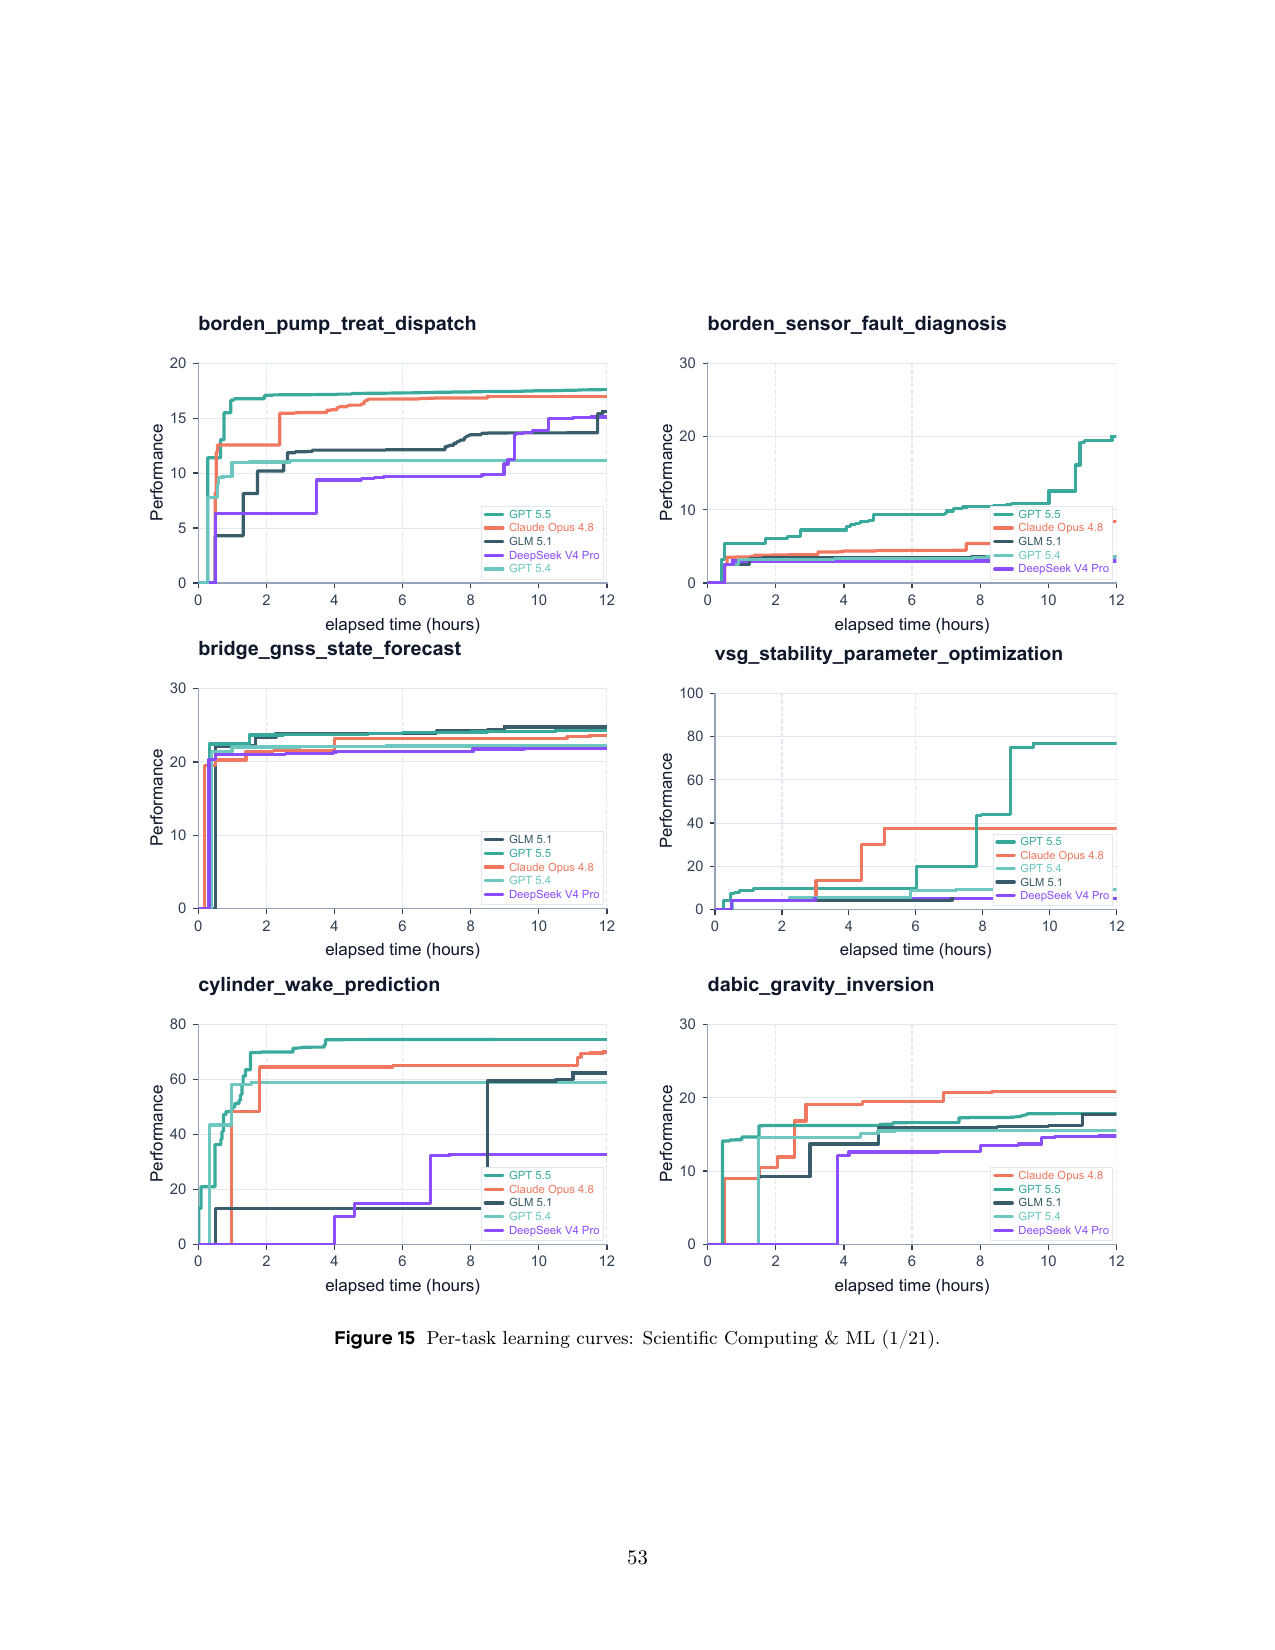
\includegraphics[width=0.32\textwidth]{figures/page-53.png}\hfill
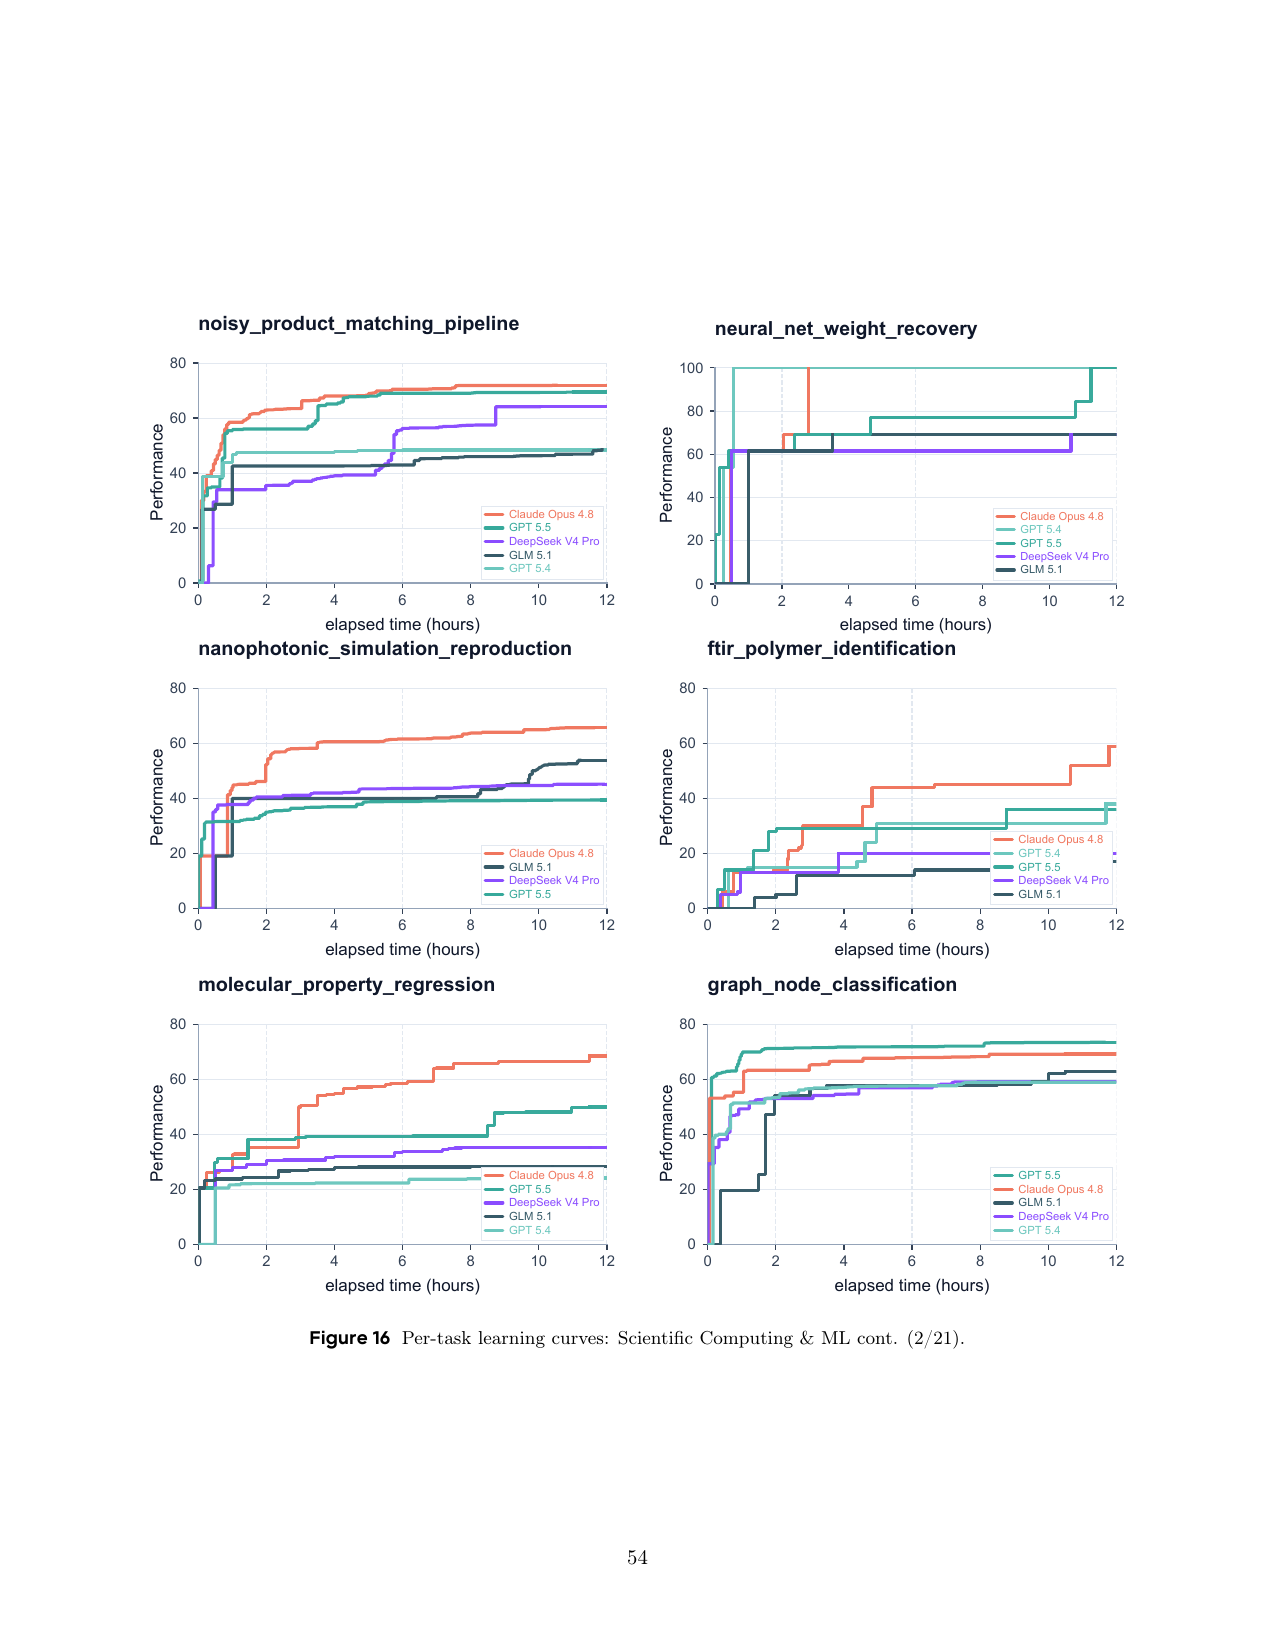
\includegraphics[width=0.32\textwidth]{figures/page-54.png}\hfill
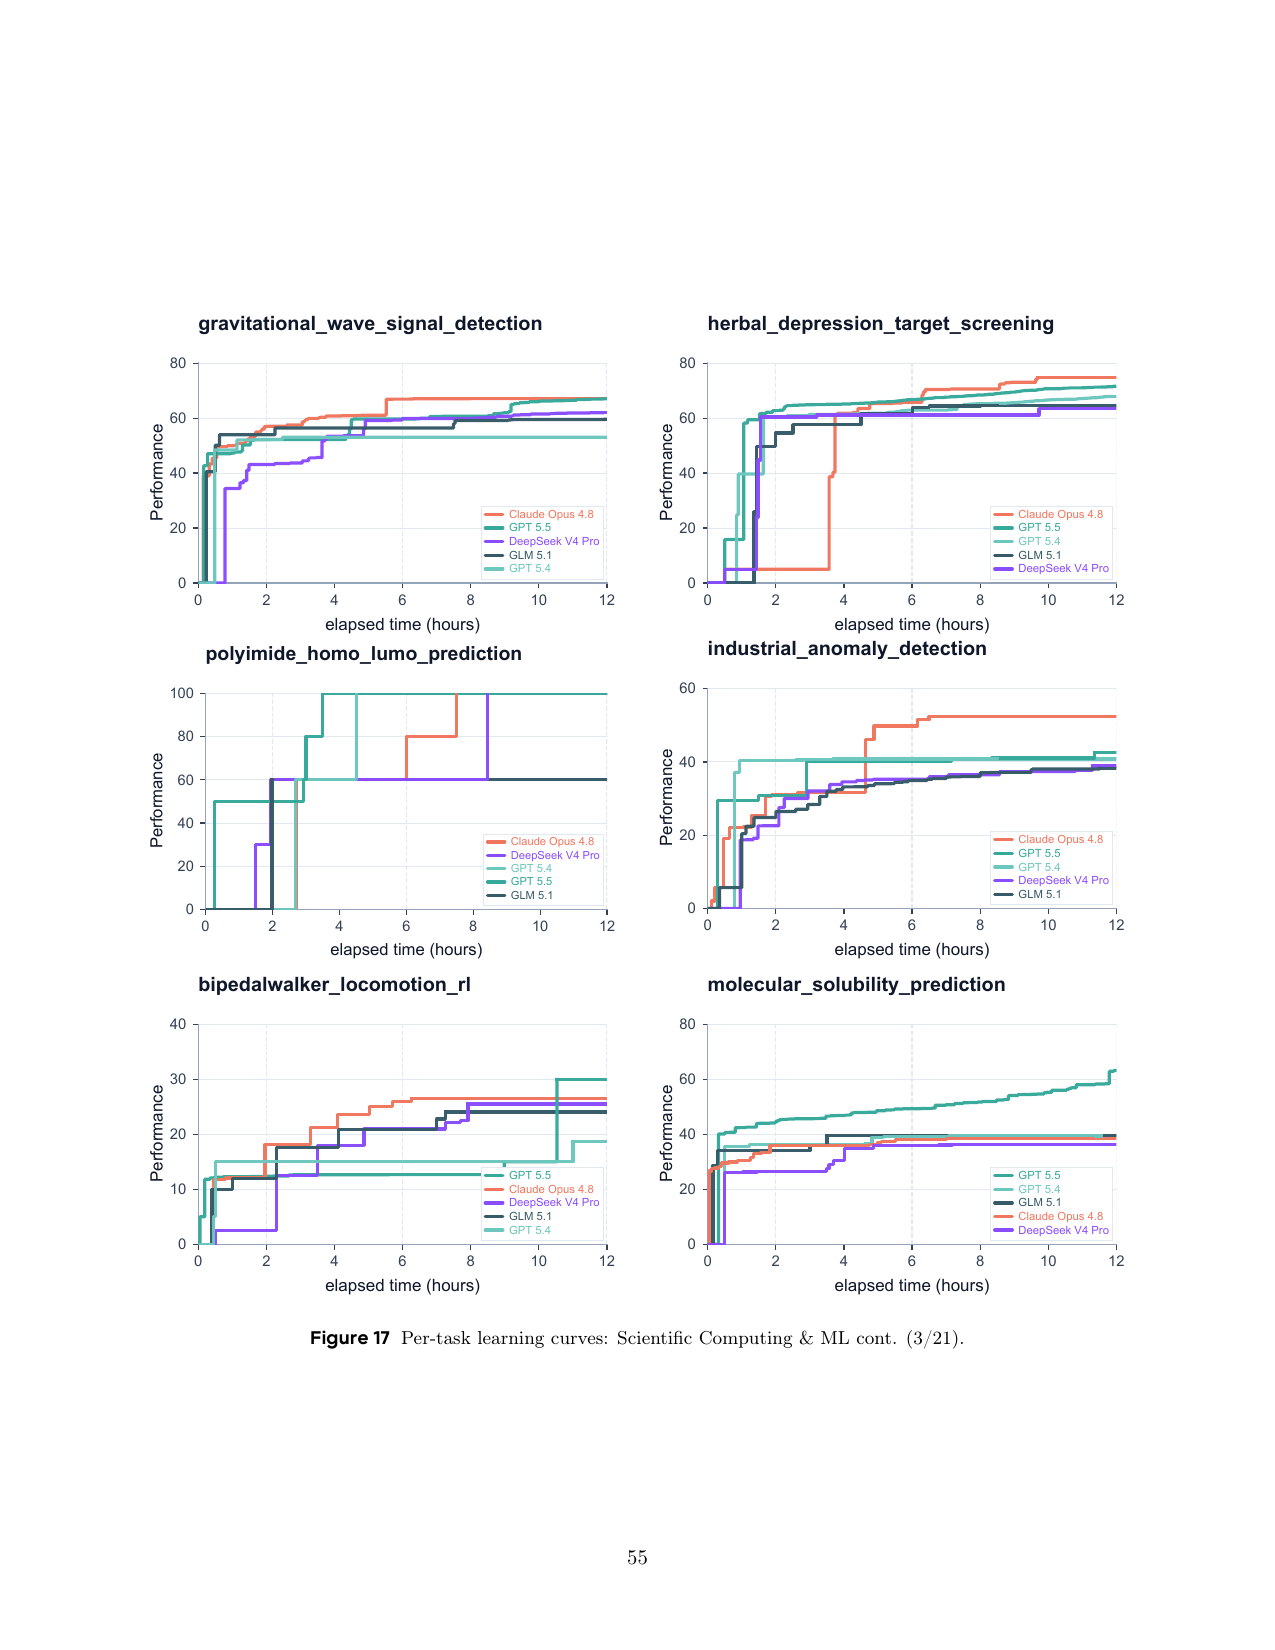
\includegraphics[width=0.32\textwidth]{figures/page-55.png}
\caption{逐任务学习曲线(节选)。完整 21 套曲线见原始论文附录 G.5。}
\label{fig:per-task-curves-1}
\end{figure}

\begin{figure}[h]
\centering
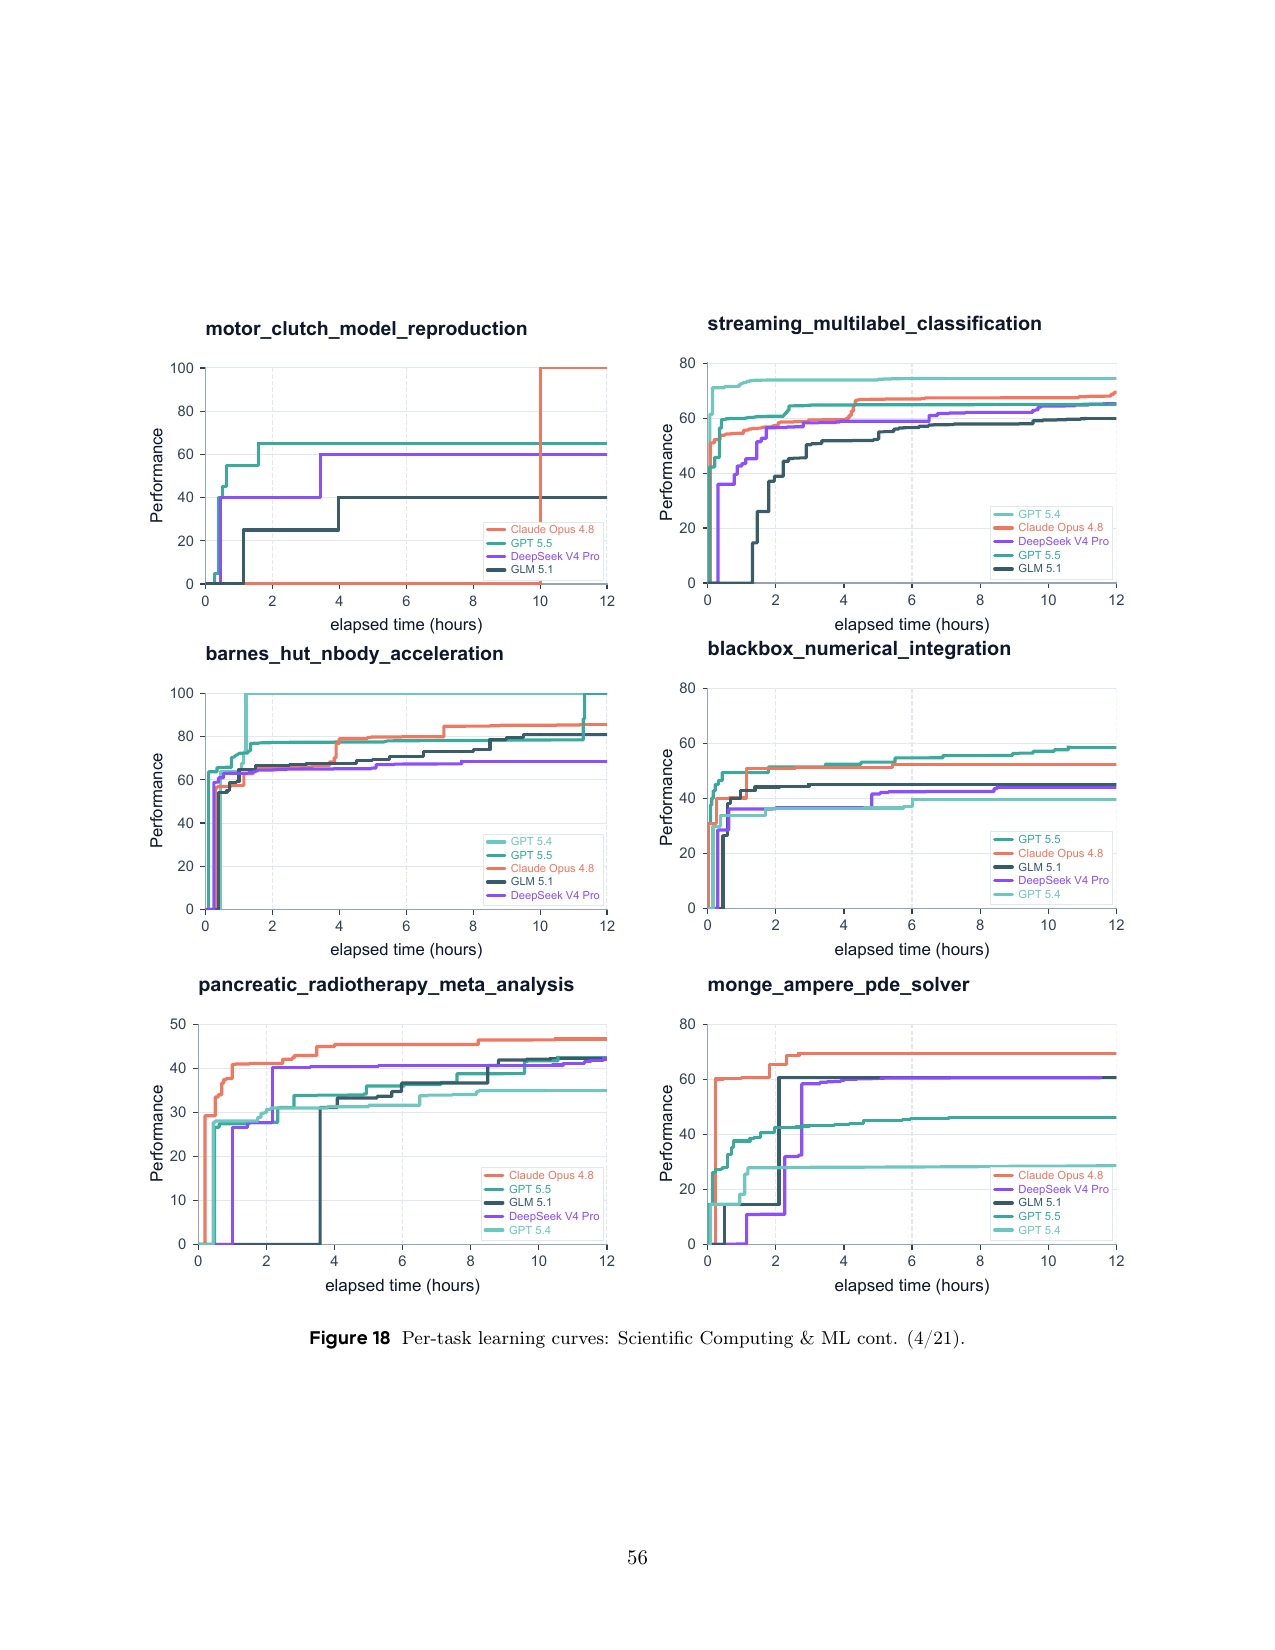
\includegraphics[width=0.32\textwidth]{figures/page-56.png}\hfill
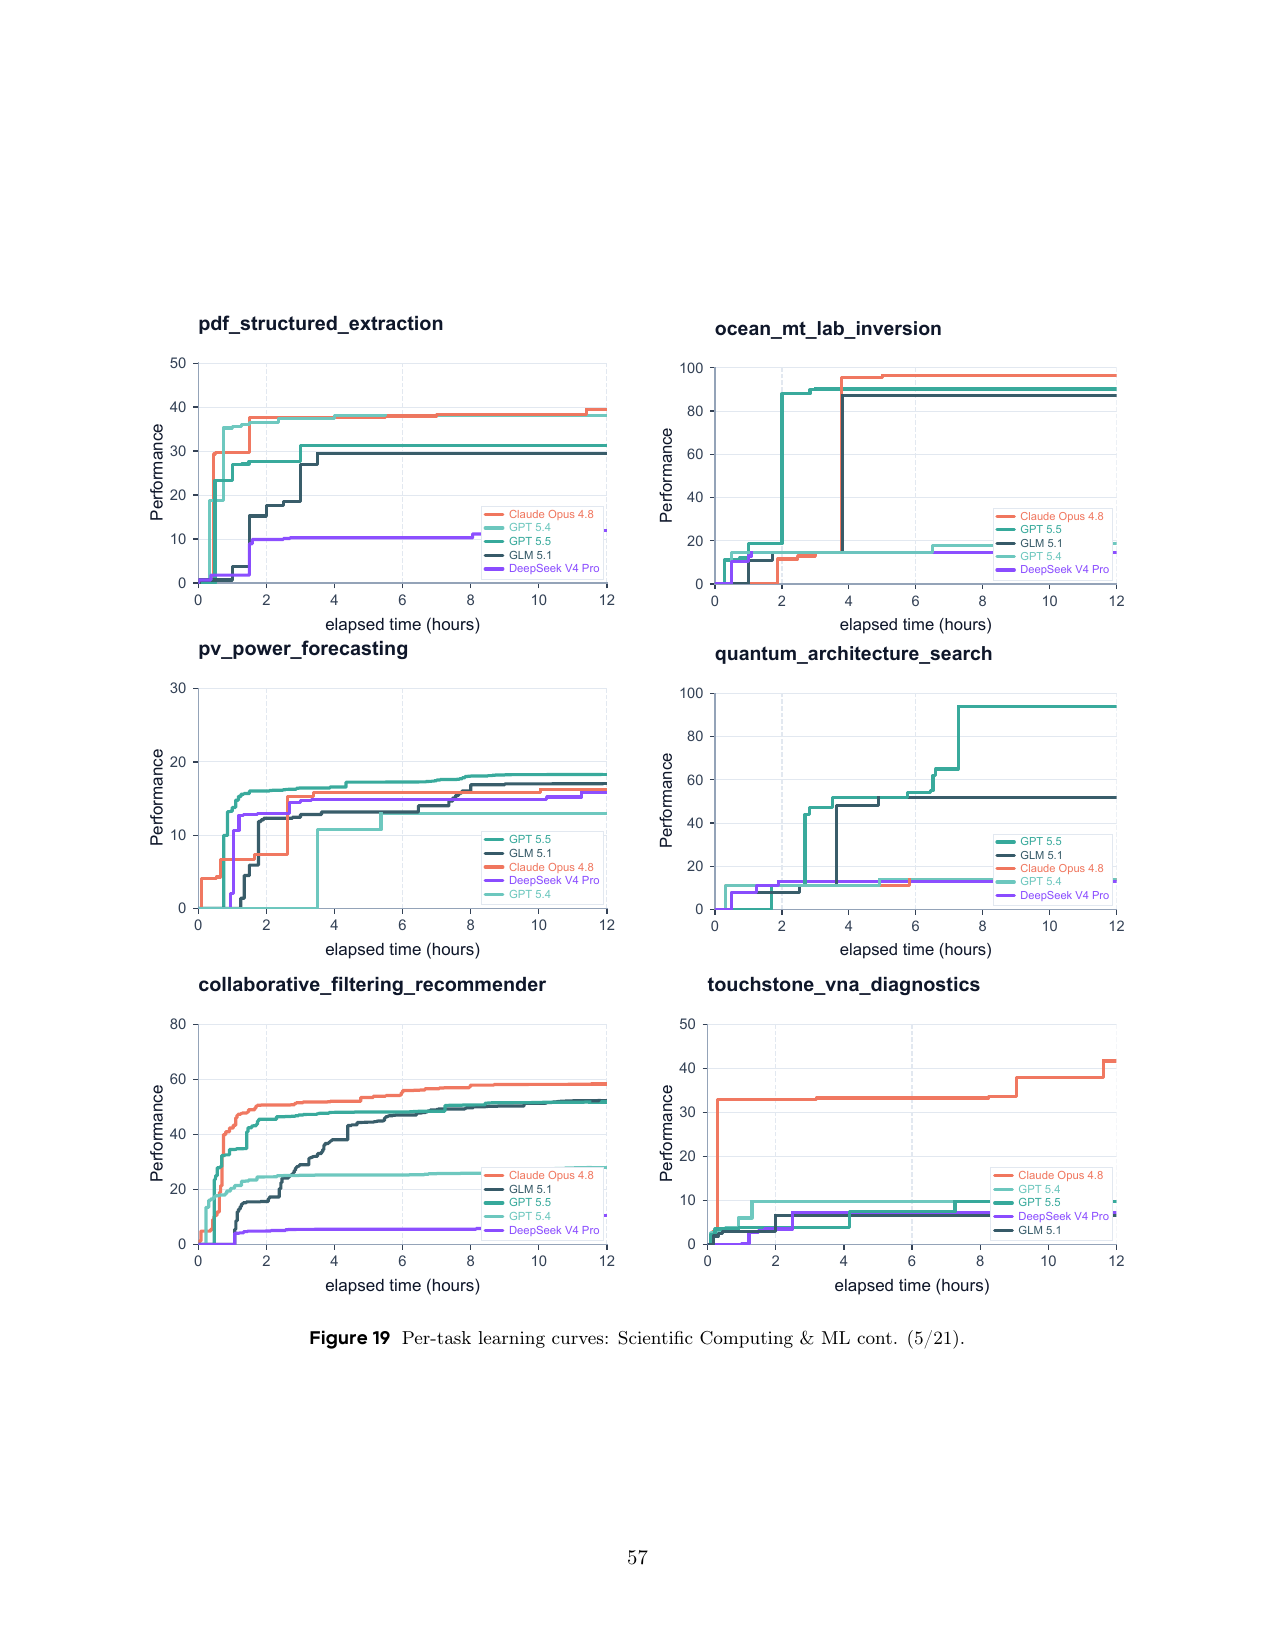
\includegraphics[width=0.32\textwidth]{figures/page-57.png}\hfill
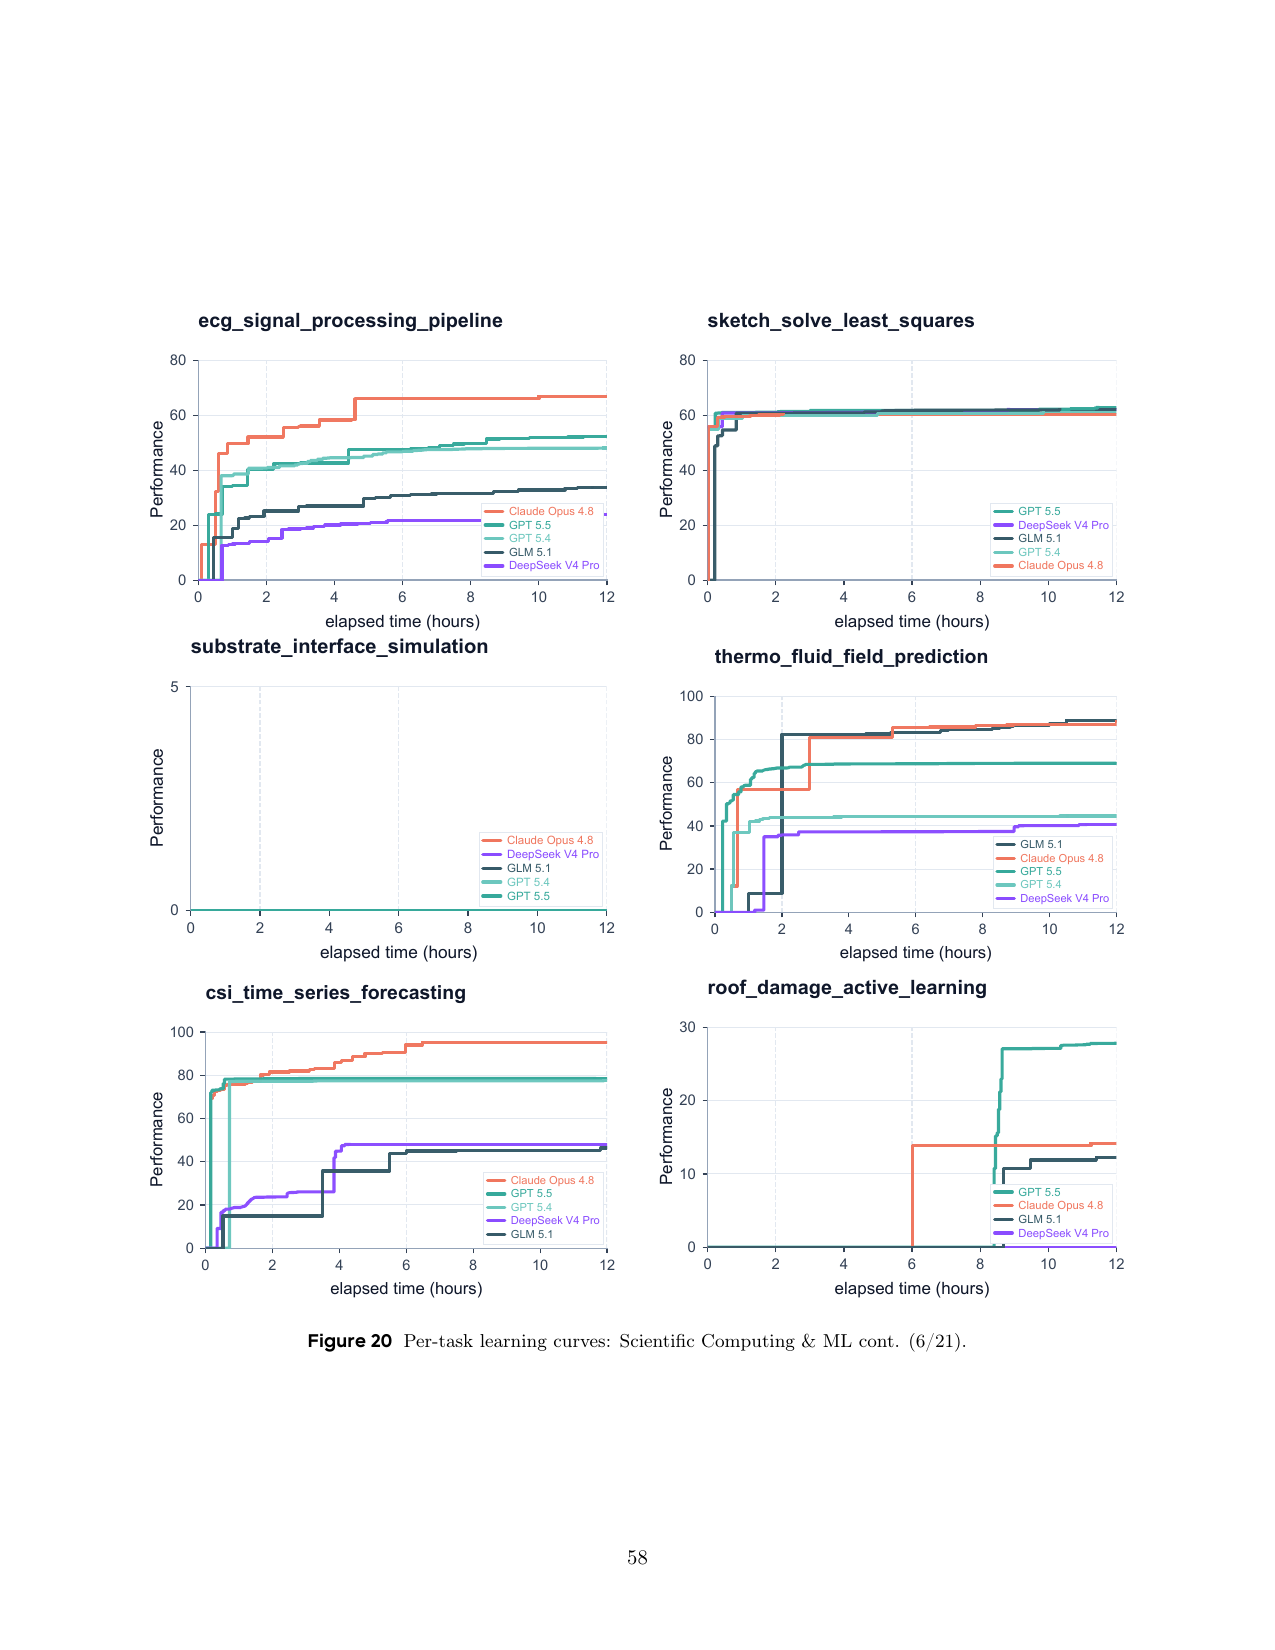
\includegraphics[width=0.32\textwidth]{figures/page-58.png}
\caption{逐任务学习曲线(科学/ML 与系统工程,节选)。}
\label{fig:per-task-curves-2}
\end{figure}

\subsection{逐任务分数表}
\label{app:score-tables}

下表给出所有任务-模型配置的分数。

\begin{table}[h]
\centering
\footnotesize
\setlength{\tabcolsep}{2pt}
\begin{tabular}{l ccccc}
\toprule
\textbf{任务(系统工程, 节选)} & \textbf{Opus 4.8} & \textbf{GPT-5.5} & \textbf{GPT-5.4} & \textbf{GLM-5.1} & \textbf{DS-V4-Pro} \\
\midrule
\texttt{codeflash\_repair\_performance} & 57.2$\pm$21.9 & \textbf{100.0*}$\pm$0.0 & --- & --- & 30.5$\pm$17.9 \\
\texttt{ffmpeg\_swscale\_reimplementation} & \textbf{21.1}$\pm$7.9 & 15.3$\pm$2.8 & 13.9$\pm$3.1 & 2.2$\pm$3.9 & 3.8$\pm$5.9 \\
\texttt{git\_rewrite\_in\_zig} & 23.1$\pm$2.2 & 18.4$\pm$0.4 & 15.4$\pm$2.4 & \textbf{23.5}$\pm$1.9 & 17.9$\pm$2.1 \\
\texttt{arc\_compiler\_runtime} & 52.0$\pm$0.1 & \textbf{72.4}$\pm$15.1 & 50.0$\pm$0.7 & 48.7$\pm$3.5 & 44.2$\pm$4.7 \\
\texttt{ann\_vector\_search\_qps} & \textbf{59.7}$\pm$2.1 & 40.7$\pm$18.8 & 50.2$\pm$17.4 & 38.3$\pm$17.5 & 23.8$\pm$3.0 \\
\texttt{rust\_multicrate\_reconstruction} & --- & \textbf{57.8}$\pm$16.8 & 21.4$\pm$3.0 & 38.5$\pm$21.4 & 23.6$\pm$2.4 \\
\texttt{dependent\_type\_checker} & \textbf{44.7}$\pm$3.7 & 24.7$\pm$21.4 & 3.8$\pm$6.7 & 1.9$\pm$3.2 & 0.0$\pm$0.0 \\
\texttt{entt\_graph\_module} & \textbf{100.0}$\pm$0.0 & 94.3$\pm$3.0 & 78.4$\pm$25.7 & \textbf{100.0}$\pm$0.0 & 92.0$\pm$10.5 \\
\texttt{stream\_processing\_engine} & \textbf{100.0}$\pm$0.0 & \textbf{100.0}$\pm$0.0 & \textbf{100.0}$\pm$0.0 & \textbf{100.0}$\pm$0.0 & \textbf{100.0}$\pm$0.0 \\
\texttt{quic\_transport\_stack} & 48.3$\pm$14.3 & \textbf{63.6}$\pm$8.9 & 47.1$\pm$16.1 & 52.5*$\pm$22.4 & 33.4$\pm$10.0 \\
\texttt{zstd\_api\_modernization} & \textbf{100.0}$\pm$0.0 & 95.8$\pm$7.2 & \textbf{100.0}$\pm$0.0 & \textbf{100.0}$\pm$0.0 & 91.7$\pm$14.4 \\
\bottomrule
\end{tabular}
\caption{系统工程任务上模型表现。值为最多三次有效运行上的均值;相邻项在至少两次有效运行时显示 $\pm s$。\textbf{加粗}为该任务最佳模型,\underline{下划线}为次佳模型,--- 表示无有效结果,$\ast$ 标记少于三次有效运行。}
\label{tab:scores-sse}
\end{table}

\begin{table}[h]
\centering
\footnotesize
\setlength{\tabcolsep}{2pt}
\begin{tabular}{l ccccc}
\toprule
\textbf{任务(科学/ML, 节选)} & \textbf{Opus 4.8} & \textbf{GPT-5.5} & \textbf{GPT-5.4} & \textbf{GLM-5.1} & \textbf{DS-V4-Pro} \\
\midrule
\texttt{capecod\_plume\_reconstruction} & \textbf{19.9}$\pm$11.1 & 16.4$\pm$5.5 & 12.6$\pm$4.6 & 10.9$\pm$2.5 & 8.8$\pm$0.4 \\
\texttt{battery\_soh\_rul\_anomaly} & \textbf{37.2}$\pm$10.7 & 30.2$\pm$14.8 & 14.7$\pm$1.8 & 18.2$\pm$4.3 & 14.0$\pm$0.6 \\
\texttt{borden\_source\_inversion} & \textbf{48.4}$\pm$7.3 & 38.5$\pm$14.3 & 8.0$\pm$1.4 & 15.1$\pm$13.7 & 38.2$\pm$3.6 \\
\texttt{cylinder\_wake\_prediction} & 66.6$\pm$4.3 & \textbf{69.9}$\pm$4.6 & 39.8$\pm$16.6 & 36.9*$\pm$36.0 & 24.2$\pm$14.6 \\
\texttt{noisy\_product\_matching\_pipeline} & \textbf{68.1}$\pm$6.5 & 64.3$\pm$6.8 & 27.1$\pm$24.7 & 44.7$\pm$3.4 & 54.2$\pm$9.1 \\
\texttt{neural\_net\_weight\_recovery} & 94.9$\pm$8.9 & \textbf{100.0*} & \textbf{100.0*}$\pm$0.0 & 69.2$\pm$0.0 & 65.4*$\pm$5.4 \\
\texttt{gravitational\_wave\_signal\_detection} & 61.5$\pm$8.1 & \textbf{64.5}$\pm$2.2 & 50.0$\pm$3.7 & 44.8$\pm$15.7 & 58.8$\pm$2.9 \\
\texttt{polyimide\_homo\_lumo\_prediction} & 86.7$\pm$23.1 & \textbf{100.0*}$\pm$0.0 & \textbf{100.0*}$\pm$0.0 & 60.0*$\pm$0.0 & 80.0*$\pm$28.3 \\
\texttt{barnes\_hut\_nbody\_acceleration} & 78.4$\pm$6.2 & \textbf{91.6}$\pm$14.5 & 87.4$\pm$15.4 & 64.1$\pm$8.5 & 67.1$\pm$2.2 \\
\texttt{csi\_time\_series\_forecasting} & \textbf{83.4}$\pm$10.4 & 76.3$\pm$2.5 & 77.3$\pm$0.2 & 44.6$\pm$3.1 & 40.4$\pm$12.3 \\
\bottomrule
\end{tabular}
\caption{科学/ML 任务上模型表现(节选)。完整表格见原文表 9。}
\label{tab:scores-ml}
\end{table}

完整 134 项任务的分数表请见原文表 8--13(对应于原文第 75--78 页),这里仅展示代表性节选以节约版面。

\subsection{致谢}
\label{app:ack}

我们感谢 UniPat 协助开发 EdgeBench 系统与软件工程部分的 13 个任务;感谢 Xiaoxing Wu、Xiang Gao、Gao Liu、Yue Yang、Wen Heng、Weinan Zhao、Mailun Gao、Zongbao Zhang 与 Yuchen Wu 在项目期间做出的有益辅助贡献;感谢 Xinkai Zhou 与 Qi Zhao 在项目期间进行的有意义的讨论;感谢 Tenglong Ao、Ao Zhang、Shengjie Luo、Zeyi Zhang、Guhao Feng、Tianle Cai、Xinrong Zhang、Yizhong Wang 与 Ruinian Chang 在 EdgeBench 项目之前进行的有意义讨论与合作。
